\documentclass{article}\usepackage[]{graphicx}\usepackage[]{color}
%% maxwidth is the original width if it is less than linewidth
%% otherwise use linewidth (to make sure the graphics do not exceed the margin)
\makeatletter
\def\maxwidth{ %
  \ifdim\Gin@nat@width>\linewidth
    \linewidth
  \else
    \Gin@nat@width
  \fi
}
\makeatother

\definecolor{fgcolor}{rgb}{0.345, 0.345, 0.345}
\newcommand{\hlnum}[1]{\textcolor[rgb]{0.686,0.059,0.569}{#1}}%
\newcommand{\hlstr}[1]{\textcolor[rgb]{0.192,0.494,0.8}{#1}}%
\newcommand{\hlcom}[1]{\textcolor[rgb]{0.678,0.584,0.686}{\textit{#1}}}%
\newcommand{\hlopt}[1]{\textcolor[rgb]{0,0,0}{#1}}%
\newcommand{\hlstd}[1]{\textcolor[rgb]{0.345,0.345,0.345}{#1}}%
\newcommand{\hlkwa}[1]{\textcolor[rgb]{0.161,0.373,0.58}{\textbf{#1}}}%
\newcommand{\hlkwb}[1]{\textcolor[rgb]{0.69,0.353,0.396}{#1}}%
\newcommand{\hlkwc}[1]{\textcolor[rgb]{0.333,0.667,0.333}{#1}}%
\newcommand{\hlkwd}[1]{\textcolor[rgb]{0.737,0.353,0.396}{\textbf{#1}}}%

\usepackage{framed}
\makeatletter
\newenvironment{kframe}{%
 \def\at@end@of@kframe{}%
 \ifinner\ifhmode%
  \def\at@end@of@kframe{\end{minipage}}%
  \begin{minipage}{\columnwidth}%
 \fi\fi%
 \def\FrameCommand##1{\hskip\@totalleftmargin \hskip-\fboxsep
 \colorbox{shadecolor}{##1}\hskip-\fboxsep
     % There is no \\@totalrightmargin, so:
     \hskip-\linewidth \hskip-\@totalleftmargin \hskip\columnwidth}%
 \MakeFramed {\advance\hsize-\width
   \@totalleftmargin\z@ \linewidth\hsize
   \@setminipage}}%
 {\par\unskip\endMakeFramed%
 \at@end@of@kframe}
\makeatother

\definecolor{shadecolor}{rgb}{.97, .97, .97}
\definecolor{messagecolor}{rgb}{0, 0, 0}
\definecolor{warningcolor}{rgb}{1, 0, 1}
\definecolor{errorcolor}{rgb}{1, 0, 0}
\newenvironment{knitrout}{}{} % an empty environment to be redefined in TeX

\usepackage{alltt}
\setlength{\parindent}{0pt} % Remove indent at new paragraphs
\setcounter{secnumdepth}{4}  % Remove section numbering at certain depth # If zero, then no numbering of sections
\setcounter{tocdepth}{4} % Determines number of subsections that will have tabs
\usepackage{tabu}
\usepackage[round,sort]{natbib}
\usepackage{fixltx2e}
\usepackage{graphicx}	% For external pictures
\usepackage{float}
\usepackage{subfig}	% Add subfigures within figures
\usepackage{verbatim}
\usepackage[colorlinks=true,linkcolor=blue,citecolor=blue,urlcolor=blue]{hyperref}
\usepackage{amssymb,amsbsy,amsmath}
\usepackage{epsfig}
\usepackage[left=3cm,top=3cm,bottom=3.5cm,right=3cm]{geometry} % For easy document margins
\usepackage{fancyhdr} % For customization of header/footer
\usepackage{adjustbox}
\usepackage{framed}
\usepackage{enumitem}
\usepackage{caption}
\numberwithin{equation}{section} % Equation numbers relative to sections
\usepackage[dvipsnames]{xcolor}

%\usepackage[usenames]{colors}
%\definecolor{darkred}{rgb}{0.545,0,0}
%\definecolor{midnightblue}{rgb}{0.098,0.098,0.439}
%\DefineVerbatimEnvironment{Sinput}{Verbatim}{fontshape=sl,formatcom={\color{midnightblue}}}
%\DefineVerbatimEnvironment{Soutput}{Verbatim}{formatcom={\color{darkred}}}
%\DefineVerbatimEnvironment{Scode}{Verbatim}{fontshape=sl,formatcom={\color{blue}}}

% ---------------------------------------------------------------------------------------------------------------------------------------

% \VignetteIndexEntry{ePort: Student performance report generation for statistics instructors}
%\VignetteEngine{knitr::knitr}
%\VignettePackage{ePort}
%\documentclass{amsart}
\newcommand{\code}[1]{{\texttt{#1}}}
\newcommand{\pkg}[1]{{\texttt{#1}}}
\newcommand{\class}[1]{{\textit{#1}}}
\newcommand{\R}{{\normalfont\textsf{R }}{}}
\IfFileExists{upquote.sty}{\usepackage{upquote}}{}
\begin{document}
\sloppy





%\SweaveOpts{prefix.string=fig,include=F,keep.source=T,eps=FALSE}

% <<echo=false>>=
% options(continue="  ")
% @
% %@% TO ELIMINATE THE "+" IN CONSECUTIVE SCRIPT LINES

\title{ePort Vignette:\\ Academic report generation for instructors}
\author{Xiaoyue Cheng, Di Cook, Lindsay Rutter, Amy Froelich}
\date{\pkg{ePort} version 0.1.0 , 2016-07-10 }
\maketitle

\tableofcontents
\setcounter{footnote}{1} \footnotetext{This \LaTeX\ vignette document is created using the \textbf{\textsf{R}} function \code{knitr} on the \textbf{\textsf{R}} package \pkg{ePort}. It is automatically downloaded with the package and can be accessed with the \textbf{\textsf{R}} command \code{vignette("ePort")}. This vignette was written by Lindsay Rutter.}  \newpage
\setlength{\parskip}{10pt} % Inter-paragraph spacing



\section{Introduction}

\subsection{Summary}

The \pkg{ePort} package provides tools for course instructors to generate electronic reports regarding student performance. Instructors can produce reports immediately after homework assignment deadlines, and use them to better understand student performance throughout the teaching semester. The goal is to allow instructors to assess and improve upon their teaching approaches in a fast response cycle.

The tools in this package will be especially beneficial for users who supervise large introductory courses. These courses often consist of multiple topics (groups of learning outcomes) that are taught by multiple instructors across multiple sections (groups of students). To accomodate the various ways that student performance can be examined for such courses, the package can generate various reports that can compare within and between topics and sections.

At its simplest, a report can be generated for one topic and one section. This would allow course coordinators to determine how well a particular section performed on a particular topic. Reports can also be generated for one topic across multiple sections, which can allow course coordinators to quickly determine how well and consistently the multiple sections performed on a topic of interest. This could be particularly insightful in cases where discrepancies in student performance are discovered between sections, especially if different instructors and/or teaching methods are being used across the sections.

In addition, we can produce reports for one unit (group of topics), either within one section or between multiple sections. This allows coordinators to assess student performance across all the learning outcomes of the combined topics that form the unit, and to quantify the consistency of how students perform across sections.

In general, both short and long versions of reports can be generated. Short versions of reports provide brief summarizations of student performance without regard to individual problems, whereas long versions of reports provide detailed summarizations of student performance for each individual problem in the assignment. Hence, long reports can also be used to confirm the suitability of assigned problems. For instance, in some courses, problems that assess the same learning outcome and are intended to be of equal difficulty levels are grouped into a question set, and each student is assigned a random subset from this set of problems. However, sometimes, an unexpected discrepancy in student performance between problems in a given quesiton set will be discovered, indicating an unintended discrepancy in the clearness or difficulty level of the problems to which students were randomly assigned. This package will allow users to efficiently find and fix such issues. 

\subsection{Installation}

\textbf{\textsf{R}} is a open source software project for statistical computing, and can be freely downloaded from the Comprehensive \textbf{\textsf{R}} Archive Network (\texttt{CRAN}) website. The link to contributed documentation on the \texttt{CRAN} website offers practical resources for an introduction to \textbf{\textsf{R}} in several languages. After downloading and installing \textbf{\textsf{R}}, the installation of additional packages is straightforward. To install the \pkg{ePort} package from \textbf{\textsf{R}}, use the command: \\

\begin{knitrout}
\definecolor{shadecolor}{rgb}{0.969, 0.969, 0.969}\color{fgcolor}\begin{kframe}
\begin{alltt}
\hlkwd{install.packages}\hlstd{(}\hlstr{"ePort"}\hlstd{)}
\end{alltt}
\end{kframe}
\end{knitrout}

\noindent
The \pkg{ePort} package should now be successfully installed. Next, to render it accessible to the current \textbf{\textsf{R}} session, simply type: \\

\begin{knitrout}
\definecolor{shadecolor}{rgb}{0.969, 0.969, 0.969}\color{fgcolor}\begin{kframe}
\begin{alltt}
\hlkwd{library}\hlstd{(ePort)}
\end{alltt}
\end{kframe}
\end{knitrout}

\subsection{Help files}
\label{sec:helpSection}

To access help pages with example syntax and documentation for the available functions of the \pkg{ePort} package, please type: \\

\begin{knitrout}
\definecolor{shadecolor}{rgb}{0.969, 0.969, 0.969}\color{fgcolor}\begin{kframe}
\begin{alltt}
\hlkwd{help}\hlstd{(}\hlkwc{package}\hlstd{=}\hlstr{"ePort"}\hlstd{)}
\end{alltt}
\end{kframe}
\end{knitrout}

To access more detailed information about a specific function in the \pkg{ePort} package, use the following help command on that function, such as: \\

\begin{knitrout}
\definecolor{shadecolor}{rgb}{0.969, 0.969, 0.969}\color{fgcolor}\begin{kframe}
\begin{alltt}
\hlkwd{help}\hlstd{(mergeSection)}
\end{alltt}
\end{kframe}
\end{knitrout}

The above command will return the help file for the function. Notice that this help file includes freestanding example syntax to illustrate how function commands are executed. This is the case in help files for most functions. The provided example code can be pasted directly into an \textbf{\textsf{R}} session.

\section{Online homework database}
\label{sec:OnlineHomework}

Amy Froelich, one of the authors of the \texttt{ePort} package, developed an online homework database that has been applied for years in a large multi-section introductory statistics course. The resulting student data from this database has been applied to the \texttt{ePort} package, and has been useful in discovering common patterns and/or problems in student learning in this course. In this section of the vignette, we will describe the configuration of this particular database, keeping in mind that a course supervisor who is interested in applying the \texttt{ePort} package to their course can do so by constructing their own online homework database in a similar format to the one described below.

\subsection{Database structure}

The online homework database consists of 184 learning outcomes, which are grouped into 26 topics. In total, the database contains 2000 questions. A given student does not receive all 2000 questions over the course of the semester. Instead, similar questions are grouped together to form 330 question sets, and a given student will receive a specified number of questions (usually one) from each of these 330 question sets.

\subsubsection{Topics}

The topics in the database cover a broad range of material that includes curriculum from Advanced Placement Statistics and popular introductory statistics textbooks. The topics are not rigidly structured around a specific textbook, and are not self-contained. Hence, course supervisors can tailor their course by selecting a subset of and/or reordering topics from the database. The full list of topic numbers and descriptions from the database is provided below in Table \ref{tab:topics}.

\begin{center}
\captionof{table}{Topic numbers and descriptions}
\label{tab:topics}
\begin{tabular} { | l | l | }
\hline \textbf{Number} & \textbf{Description} \\
\hline
01 & Data \\
\hline
02  & Descriptive Statistics for a Single Categorical Variable \\
\hline
03 & Descriptive Statistics for a Single Quantitative Variable \\
\hline
04 & Descriptive Statistics for a Contingency Table \\
\hline
05 & Descriptive Statistics for a Single Quantitative Variable between Groups \\
\hline
06 & Normal Distribution \\
\hline
07 & Descriptive Statistics for a Scatterplot \\
\hline
08 & Descriptive Linear Regression \\
\hline
09 & Samples and Surveys \\
\hline
10 & Experiments \\
\hline
11 & Randomness and Probability \\
\hline
12 & Introduction to Probability and Events \\
\hline
13 & Introduction to Random Variables \\
\hline
14 & Binomial and Poisson Distributions \\
\hline
15 & Sampling Distribution for the Sample Proportion \\
\hline
16 & Confidence Intervals for the Population Proportion \\
\hline
17 & Hypothesis Tests for the Population Proportion \\
\hline
18 & Sampling Distribution for the Sample Mean \\
\hline
19 & Confidence Intervals for the Population Mean \\
\hline
20 & Hypothesis Tests for the Population Mean \\
\hline
21 & Inference for the Difference in Two Population Proportions \\
\hline
22 & Inference for the Difference in Two Population Means \\
\hline
23 & Inference for the Mean Difference (Paired Samples) \\
\hline
24 & Goodness of Fit Tests \\
\hline
25 & Inference for Contingency Tables \\
\hline
26 & Inference for Simple Linear Regression \\
\hline
\end{tabular}
\end{center}

\subsubsection{Learning outcomes}

Each topic contains learning outcomes, which are a list of statements that describe what a student is expected to understand after completing the topic. Learning outcomes form the main structure of the electronic assessment model of \texttt{ePort}. The average topic contains about seven learning outcomes. As an example, the learning outcomes for \texttt{Topic 03} are provided in List \hyperref[sec:lo]{1} below.

\newpage
\centerline{List 1: Learning outcomes for Topic 03}
\vspace{-2mm}
\begin{framed}
\begin{enumerate}[label=\Alph*.]
\label{sec:lo}
\item Use standardizing to determine how many standard deviations an observation is away from the mean value.
\item Use z-scores to compare observations for different quantitative variables.
\item Explain how standardizing affects the shape, center, and variability of the distribution of a quantitative variable.
\item Determine which quantitative variables could be modeled using the normal distribution by interpreting graphical representations of the variable.
\item Apply the 68-95-99.7 Rule to any quantitative variable with a normal distribution.
\item Find percentile or area values for any given observation from a normal distribution.
\item Find the value of an observation when given a percentile or area value from the normal distribution.
\end{enumerate}
\end{framed}

\subsubsection{Question types}

The majority of the questions in the database include real data examples that cover diverse application areas, excepting business. The questions are time-tested in that they have continuously been edited and improved upon after evaluating student responses time and again. The majority of these questions also include feedback, which can be correct/incorrect feedback or answer-specific feedback. There are seven types of questions, which are displayed in Table \ref{tab:questionTypes}.

\begin{center}
\captionof{table}{Seven types of questions in the database}
\label{tab:questionTypes}
\begin{tabular} { | l | l | l |}
\hline \textbf{Abbreviation} & \textbf{Type} & \textbf{Possible Points} \\
\hline
TF & True/False & 1 \\
\hline
MC & Multiple Choice & 1 \\
\hline
MU & Multiple Answer & 1 \\
\hline
MA & Matching & Number of Matches \\
\hline
FB & Fill in the Blank & Number of Blanks \\
\hline
JS & Jumbled Sentence & Number of Blanks \\
\hline
CA & Calculation & 1 \\
\hline
\end{tabular}
\end{center}

In each of the seven boxes that follow, we provide an example question and example solution. For demonstration purposes, each box covers a different question type in the database. \\

%\centerline{\textbf{Example TF:}}
\begin{framed}
\textbf{Example TF:}

Does regular exercise lead to higher VO$_2$ max? VO$_2$ max is the maximum amount of oxygen in millimeters, one can use in one minute per kilogram of body mass. A random sample of 20 college age women was selected. Each student was asked whether or not they exercised regularly (at least 30 minutes of aerobic exercise 3 times a week). The VO$_2$ max for each student was also taken. This is an observational study.

a. True\\
b. False

Correct answer: a
\end{framed}

\begin{framed}
\textbf{Example MC:}

The z-score for a particular observation is z = -3.1. This means the observation is:

a. 3.1 standard deviations above the mean\\
b. 3.1 standard deviations below the mean\\
c. 3.1 units above the mean\\
d. 3.1 units below the mean

Correct answer: b
\end{framed}

\begin{framed}
\textbf{Example MU:}

Which of the following characteristics of pie is/are quantitative variables? Choose ALL that apply.

a. Calorie count\\
b. Number of cups of flour used\\
c. Type of pie (pecan, blueberry, etc)\\
d. Brand of sugar used

Correct answers: a and b
\end{framed}

\begin{framed}
\textbf{Example MA:}

An ultramarathon is a foot race that is longer than 26.2 miles. Doctors have found that people who run an ultramarathon are at increased risk for developing respiratory infections after the race. Doctors beleive that taking vitamin C the 10 days before and the 10 days after the race would reduce the incidence of respiratory infections in the ultramarathon runners. To test their hypothesis, 20 runners were randomly assigned into two groups of 10 runners each. One group was given the same dose of vitamin C, in pill form, for 10 days before and 10 days are the race and the other group was given a sugar pill. Ten days after the race, the two groups were studied to determine how many of the runners in each group developed a respiratory infection. Match the ordered terms (1-4) to the correct description (a-d).

1. Experimental units\\
2. Response variable\\
3. Factor\\
4. Treatments

a. 20 ultramarathon runners\\
b. The use of vitamin C by ultramarathon runners\\
c. Whether or not the runner developed a respiratory infection\\
d. Vitamin C, Sugar pill

Correct answer: a, c, b, d
\end{framed}

\begin{framed}
\textbf{Example FB:}

Fill in the blank with the correct number: Assume the length of female humpback whales can be modeled with a normal distribution with a mean of 13.7 meters and a standard deviation of 0.5 meters. According to the Empirical Rule or 68-95-99.7 Rule, \underline{\hspace{2cm}} percent of female humpback whales will have a length between 13.2 meters and 14.2 meters.

Correct matches: 68 or 68\%
\end{framed}

\begin{framed}
\textbf{Example JS:}

All other things being equal, a \underline{\hspace{2cm}} confidence interval for a population proportion will be wider than a \underline{\hspace{2cm}} confidence interval for the same population proportion.

Correct answer: 95\%, 90\%
\end{framed}

\begin{framed}
\textbf{Example CA:}

The regression line for predicting the value of a variable $y$ from the value of a variable $x$ is as follows:

$y = 1.25 + 0.5x$

Use this equation to predict the value of $y$ when the value of $x$ is 188. Round your final answer to 2 decimal places.

Correct answer: 95.25
\end{framed}

\subsubsection{Question sets}

A question set consists of a set of questions that all have the same format (are all one of the seven possible question types), and all cover the same component of a learning outcome. Question sets allow for different students to be presented with different subsets of similar questions. The number of questions from a given question set that are to be presented to each student is specified, and the questions are selected at random. There is at least one question set per learning outcome, and there is no connection between question sets.

\subsection{Report generation outline}

A diagram of the report generation process can be seen in Figure \ref{fig:overviewFigure}. Blue boxes represent external software (\texttt{Respondus} and \texttt{Blackboard}) that must be used along with \texttt{ePort}. Green boxes represent the three file types that must be provided as input in order for \texttt{ePort} to generate reports. Red boxes represent functions within \texttt{ePort} that are then used to produce the reports.

\begin{center}
\captionsetup{width=\textwidth}
\fbox{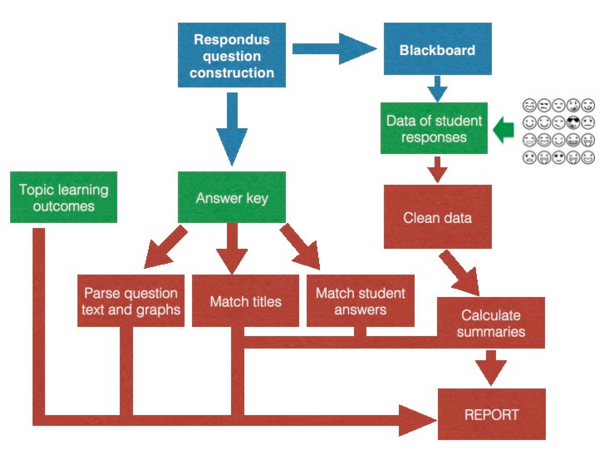
\includegraphics[width=\textwidth]{imageLayout.png}}
\captionof{figure}{Overview of report generation. Database questions are constructed in \texttt{Respondus}. Students can access and submit their assignments on \texttt{Blackboard}. The student responses are saved to the data file, one of the three input files for \texttt{ePort}. The other two input files needed for \texttt{ePort} are the answer key file and the topic learning outcomes file. The student data file must be parsed/cleaned in \texttt{ePort}, and the question titles in the answer key file can then be matched to those in the student data file. Answer texts and graphs alike must be parsed in \texttt{ePort} for the report to provide student performance summaries on individual questions. The student topic learning outcome file is also used for analyses on how students performed at the learning outcome level. Student performance summaries using information from these input files is then performed in \texttt{ePort}, and collected into reports.}
\label{fig:overviewFigure}
\end{center}

\subsubsection{External software - Respondus}
\label{sec:ResSection}

External software that must be used for \texttt{ePort} to generate the reports are represented in the blue boxes of Figure \ref{fig:overviewFigure}. As this figure shows, the database questions are constructed in the software \texttt{Respondus}. More information about \texttt{Respondus} can be found on their \href{https://www.respondus.com/}{website}.

It is important to code question titles in \texttt{Respondus} in a format that will allow all database questions to be identified and searched later in the \texttt{ePort} assessment model by topic, learning outcome, question type, and question set. That way, summaries of student performance at each of these levels can be performed and published in the reports. An example of a coded question title is shown below:

\begin{framed}
Example question title: \textbf{\textcolor{Red}{T16}.\textcolor{YellowOrange}{A}.\textcolor{YellowGreen}{A}.\textcolor{Green}{04-1}.\textcolor{blue}{1}.\textcolor{RedViolet}{MC}.\textcolor{VioletRed}{1}}

\textbf{\textcolor{Red}{T16}}: Topic 16\\
\textbf{\textcolor{YellowOrange}{A}}: Learning Outcome A for Topic 16\\
\textbf{\textcolor{YellowGreen}{A}}: Question Set A for Topic 16\\
\textbf{\textcolor{Green}{04-1}}: Question Set A for Topic 16 has 4 questions, and 1 is randomly assigned to each student\\
\textbf{\textcolor{blue}{1}}: All questions in Question Set A for Topic 16 are worth 1 point\\
\textbf{\textcolor{RedViolet}{MC}}: All questions in Question Set A for Topic 16 are in multiple choice format\\
\textbf{\textcolor{VioletRed}{1}}: Question label of this particular question from Question Set A for Topic 16\\
\vspace{-3mm}
\end{framed}

\subsubsection{External software - Blackboard}

As seen in Figure \ref{fig:overviewFigure}, once the database has been constructed in \texttt{Respondus}, we can upload it to \texttt{Blackboard}. More information about \texttt{Blackboard} can be found on their \href{http://www.blackboard.com/}{website}.

Typically, assignments on \texttt{Blackboard} can be made available to students on the first day the topic is introduced in lecture, and closed a set number of days after the topic is concluded in lecture. Each student can access their assignment over the course of as many sittings as needed, saving their work each time, but they can only submit their assignment once before the deadline. Once the deadline of the assignment has passed, students have access to answers and feedback for their set of questions. 

\subsubsection{Input files}

The three necessary input files for \texttt{ePort} to generate reports are represented in green in Figure \ref{fig:overviewFigure}. A file that enumerates the learning outcomes is required; an example of this type of file has already been displayed in List \hyperref[sec:lo]{1}. An answer key file is also required, and can be generated from the database in \texttt{Respondus}. The third required file consists of the answers that students submit when they complete their assignments on \texttt{Blackboard}.

\subsubsection{Parsing input files}

The functions needed to transform input files to final report files are represented in red in Figure \ref{fig:overviewFigure}. There are simple cleaning procedures that must be applied to the student response data files from \texttt{Blackboard}. One task that must then get done here is matching student answers from the cleaned student response data file to possible answer choices in the answer key from \texttt{Respondus}. This step simultaneously requires that the questions that a particular student received at random from each question set are successfully matched to the corresponding question titles in the answer key from \texttt{Respondus}.

The final reports consist of data summaries, graphics, and analyses regarding how students performed on the assignments. As will later be explained in more detail, some report types have more verbose versions, which include individual summaries for each question in the topic of interest. This means that it is not only the text, but also any graphs and equations that must be parsed in the answer key file. Doing so allows for the verbose reports to publish all components of a given question, such as relevant graphics, equations, and text, in the same way that it had been presented to students. The analysis of student performance for that question can then also be displayed alongisde the complete question itself.

\section{Example data}

A directory that contains example data is automatically installed with the \texttt{ePort} package. The name of this directory is \texttt{extdata}. Understanding the location, layout, and content of the \texttt{extdata} directory will be necessary to continue with the examples provided in the vignette.

The absolute pathway to the \texttt{extdata} directory on your local computer can be determined by typing the following command into the \textbf{\textsf{R}} console: \\

\begin{knitrout}
\definecolor{shadecolor}{rgb}{0.969, 0.969, 0.969}\color{fgcolor}\begin{kframe}
\begin{alltt}
\hlkwd{system.file}\hlstd{(}\hlstr{"inst/extdata/"}\hlstd{,} \hlkwc{package} \hlstd{=} \hlstr{"ePort"}\hlstd{)}
\end{alltt}
\end{kframe}
\end{knitrout}

\section{Generating Reports}

Currently, the \pkg{ePort} package offers six report types, depending on what the user is trying to compare and analyze about student performance. The same function \texttt{makeReport()} is used to generate each of these six report types; however, the input parameter \texttt{reportType} to the function will be different depending on which of the six report types the user wishes to run. It is most efficient for the user to hard-code in the \texttt{reportType} parameter. For that reason, below is a reference box for the six types of string options (in quotes) that can be used for the \texttt{reportType} parameter, depending on which of the six report types the user will run: 
\begin{framed}
\begin{itemize}
\vspace{-3mm}
\item One topic for one section - short version (``secTopicShort")
\item One topic for one section - long version (``secTopicLong")
\item One topic comparing multiple sections - short version (``crossSecTopicShort")
\item One topic comparing multiple sections - long version (``crossSecTopicLong")
\item One unit (group of topics) for one section (``secUnit")
\item One unit (group of topics) comparing multiple sections (``crossSecUnit")
\end{itemize}
\end{framed}

This information regarding the parameter options of the six report types can also be obtained by running \texttt{help(makeReport)}. In the next parts of the vignette, we will demonstrate how to produce each of the six report types, and, along the way, we will hard code each of the \texttt{reportType} parameter options.

\subsection{One topic for one section - short version}
\label{sec:oneTopicSectionShort}

An instructor may be motivated to generate a short report for one topic and one section if they are seeking answers to the following types of questions:

\begin{enumerate}
\item \textit{Overall, how did this section of students do on this homework assignment?}
\item \textit{Which students from this section scored poorly overall on this homework assignment?}
\item \textit{Are there any question sets for this topic that this section of students found easy or difficult?}
\end{enumerate}

\subsubsection{Code}
\label{sec:codeOnce}

We start by demonstrating how to generate the electronic report for one section one topic. This demonstration will use the example input files provided in the previously-described \texttt{extdata} directory, and will output the report to the \texttt{OutputFiles} subdirectory of the \texttt{extdata} directory. If you have not modified anything in the \texttt{extdata} directory, then the \texttt{OutputFiles} subdirectory should be empty, as we have not generated any example reports yet. 

In this demonstration, we will create a report for \texttt{Topic 06} and section \texttt{A}. Like any individual report, we will require three input files (an answer key file, a data file, and a learning outcome file). There should be three example answer key files in the subdirectory \texttt{KeyFiles} (\texttt{Topic06.Questions.htm}, \texttt{Topic07.Questions.htm}, and (\texttt{Topic08.Questions.htm}), and we will use the \texttt{Topic06.Questions.htm} file. Additionally, there should be twelve example data files in the subdirectory \texttt{DataFiles} (\texttt{Topic06.A.csv}, \texttt{Topic06.B.csv}, \texttt{Topic06.C.csv}, \texttt{Topic07.A.csv}, \texttt{Topic07.B.csv}, \texttt{Topic07.C.csv}, \texttt{Topic08.A.csv}, \texttt{Topic08.B.csv}, and \texttt{Topic08.C.csv}), and we will use the \texttt{Topic06.A.csv} file. Lastly, there should be three example learning outcome files in the subdirectory \texttt{LOFiles} (\texttt{Topic06.Outcomes.txt}, \texttt{Topic07.Outcomes.txt}, and \texttt{Topic08.Outcomes.txt}), and we will use the \texttt{Topic06.Outcomes.txt} file.

The block of code we will use to generate our report for \texttt{Topic 06} and section \texttt{A} is shown in the code block below. If this is your first time reading through the vignette, it is recommended that you do \textbf{not} run this code block all at once just yet. Instead, this code block is designed to provide you with an overview of the procedure; we will discuss each line of the code afterward. \\

\begin{knitrout}
\definecolor{shadecolor}{rgb}{0.969, 0.969, 0.969}\color{fgcolor}\begin{kframe}
\begin{alltt}
\hlstd{keyHTM} \hlkwb{=} \hlkwd{system.file}\hlstd{(}\hlstr{"inst/extdata/KeyFiles/Topic06.Questions.htm"}\hlstd{,} \hlkwc{package} \hlstd{=}
  \hlstr{"ePort"}\hlstd{)}

\hlkwd{refineKey}\hlstd{(keyHTM)}

\hlstd{keyPath} \hlkwb{=} \hlkwd{gsub}\hlstd{(}\hlstr{"htm$"}\hlstd{,} \hlstr{"txt"}\hlstd{, keyHTM)}

\hlstd{dataPath} \hlkwb{=} \hlkwd{system.file}\hlstd{(}\hlstr{"inst/extdata/DataFiles/Topic06/Topic06.A.csv"}\hlstd{,} \hlkwc{package} \hlstd{=}
  \hlstr{"ePort"}\hlstd{)}

\hlkwd{rewriteData}\hlstd{(dataPath)}

\hlstd{loPath} \hlkwb{=} \hlkwd{system.file}\hlstd{(}\hlstr{"inst/extdata/LOFiles/Topic06.Outcomes.txt"}\hlstd{,} \hlkwc{package} \hlstd{=} \hlstr{"ePort"}\hlstd{)}

\hlstd{outPath} \hlkwb{=} \hlkwd{system.file}\hlstd{(}\hlstr{"inst/extdata/OutputFiles"}\hlstd{,} \hlkwc{package} \hlstd{=} \hlstr{"ePort"}\hlstd{)}

\hlkwd{makeReport}\hlstd{(}\hlkwc{keyFile} \hlstd{= keyPath,} \hlkwc{dataFile} \hlstd{= dataPath,} \hlkwc{loFile} \hlstd{= loPath,} \hlkwc{outFile} \hlstd{=}
  \hlstd{outPath)}
\end{alltt}
\end{kframe}
\end{knitrout}

Now that we have seen the entire code required for this procedure, we briefly explain each step of the above code block. Here, we recommend that you follow along by actively running each piece of code, as will be demonstrated below. The first line from the code block is where we save the absolute pathway of the answer key. Here, we save it to a string variable called \texttt{keyHTM}. \\

\begin{knitrout}
\definecolor{shadecolor}{rgb}{0.969, 0.969, 0.969}\color{fgcolor}\begin{kframe}
\begin{alltt}
\hlstd{keyHTM} \hlkwb{=} \hlkwd{system.file}\hlstd{(}\hlstr{"inst/extdata/KeyFiles/Topic06.Questions.htm"}\hlstd{,} \hlkwc{package} \hlstd{=}
  \hlstr{"ePort"}\hlstd{)}
\end{alltt}
\end{kframe}
\end{knitrout}

Second, we must parse and clean the .htm answer key file, and convert it to plain text format. We do this by calling the \texttt{refineKey()} function of \texttt{ePort} on the .htm answer key file. By running the line below, we will create the cleaned .txt file: \\

\begin{knitrout}
\definecolor{shadecolor}{rgb}{0.969, 0.969, 0.969}\color{fgcolor}\begin{kframe}
\begin{alltt}
\hlkwd{refineKey}\hlstd{(keyHTM)}
\end{alltt}
\end{kframe}
\end{knitrout}

By default, the \texttt{refineKey()} function will place the cleaned .txt file into the same directory as the original .html file, and with the same name. Hence, if the  you navigate to the \texttt{extdata} directory and its \texttt{KeyFiles} subdirectory, you should now see the new and cleaned .txt file we just created, \texttt{Topic06.Questions.txt}.

Our third step is to save the absolute pathway of this new and cleaned .txt answer key. Below, we save it to a string variable called \texttt{keyPath}. \\

\begin{knitrout}
\definecolor{shadecolor}{rgb}{0.969, 0.969, 0.969}\color{fgcolor}\begin{kframe}
\begin{alltt}
\hlstd{keyPath} \hlkwb{=} \hlkwd{gsub}\hlstd{(}\hlstr{"htm$"}\hlstd{,} \hlstr{"txt"}\hlstd{, keyHTM)}
\end{alltt}
\end{kframe}
\end{knitrout}

Now that we have the absolute path of our cleaned .txt answer key, our fourth step is to define the absolute pathway of our data file. We save this to a variable called \texttt{dataPath}. \\

\begin{knitrout}
\definecolor{shadecolor}{rgb}{0.969, 0.969, 0.969}\color{fgcolor}\begin{kframe}
\begin{alltt}
\hlstd{dataPath} \hlkwb{=} \hlkwd{system.file}\hlstd{(}\hlstr{"inst/extdata/DataFiles/Topic06/Topic06.A.csv"}\hlstd{,} \hlkwc{package} \hlstd{=}
  \hlstr{"ePort"}\hlstd{)}
\end{alltt}
\end{kframe}
\end{knitrout}

After this, our fifth step is to prime the data file to be compatible with steps later down the pipeline of generating the reports. We do this by running the \texttt{rewriteData()} function of \texttt{ePort} on the data file. This function parses through the data file, and modifies certain trivial character issues that would otherwise cause a problem when running the reports. For more details about the specific process, please consider running a help command on the function. Below, we rewrite the data file: \\

\begin{knitrout}
\definecolor{shadecolor}{rgb}{0.969, 0.969, 0.969}\color{fgcolor}\begin{kframe}
\begin{alltt}
\hlkwd{rewriteData}\hlstd{(dataPath)}
\end{alltt}
\end{kframe}
\end{knitrout}

Upon running the above code snippet, you do not obtain a new file. Instead, the original file is overwritten. For this reason, you might inadvertantly run the function \texttt{rewriteData()} on a certain data file more than once, not remembering whether or not you have already converted it. It should not be a problem to run the function any number of times; you would simply receive a message that reads something like: ``Note: \texttt{Topic06.A.csv} was already successfully converted to usable format."

Our sixth step is to save the absolute pathway of our learning outcome file. Below, we save this path to a variable called \texttt{loPath}. \\

\begin{knitrout}
\definecolor{shadecolor}{rgb}{0.969, 0.969, 0.969}\color{fgcolor}\begin{kframe}
\begin{alltt}
\hlstd{loPath} \hlkwb{=} \hlkwd{system.file}\hlstd{(}\hlstr{"inst/extdata/LOFiles/Topic06.Outcomes.txt"}\hlstd{,} \hlkwc{package} \hlstd{=} \hlstr{"ePort"}\hlstd{)}
\end{alltt}
\end{kframe}
\end{knitrout}

After that, the seventh step is to specify our desired output directory. This is the absolute pathway of where the reports should be saved. Below, we create a variable called \texttt{outPath} to specify that we want to output our report to the \texttt{OutputFiles} subdirectory. \\

\begin{knitrout}
\definecolor{shadecolor}{rgb}{0.969, 0.969, 0.969}\color{fgcolor}\begin{kframe}
\begin{alltt}
\hlstd{outPath} \hlkwb{=} \hlkwd{system.file}\hlstd{(}\hlstr{"inst/extdata/OutputFiles"}\hlstd{,} \hlkwc{package} \hlstd{=} \hlstr{"ePort"}\hlstd{)}
\end{alltt}
\end{kframe}
\end{knitrout}

Now that we have primed our three input files (cleaned answer key, data file, and learning outcomes file) and specified our output directory, our last step is to generate the report using the \texttt{makeReport()} function. \\

\begin{knitrout}
\definecolor{shadecolor}{rgb}{0.969, 0.969, 0.969}\color{fgcolor}\begin{kframe}
\begin{alltt}
\hlkwd{makeReport}\hlstd{(}\hlkwc{keyFile} \hlstd{= keyPath,} \hlkwc{dataFile} \hlstd{= dataPath,} \hlkwc{loFile} \hlstd{= loPath,} \hlkwc{outFile} \hlstd{=}
  \hlstd{outPath)}
\end{alltt}
\end{kframe}
\end{knitrout}

Upon running this code, you will receive a message and menu (as shown below). We received this menu because we did not specify a value for the \texttt{reportType} parameter. The menu automatically appears in such circumstances to remind users that, as already mentioned, the \texttt{makeReport()} function can produce any one of six reports, and hence we cannot make any report at all until we make that specification.

\begin{framed}
\vspace{2mm}
Please enter integer (1-6) corresponding to desired report type below.

Note: If running many reports, it is more efficient to exit now and hard-code the reportType parameter. See help(makeReport).

1: One topic for one section - short version (``secTopicShort")\\
2: One topic for one section - long version (``secTopicLong")\\
3: One topic comparing multiple sections - short version (``crossSecTopicShort")\\
4: One topic comparing multiple sections - long version (``crossSecTopicLong")\\
5: One unit (group of topics) for one section (``secUnit")\\
6: One unit (group of topics) comparing multiple sections (``crossSecUnit")
\end{framed}

Since we wish to generate the type of report that is the short version of one topic for one section, then we can type the number \texttt{1} into the menu console. If we do so, then the report will be generated. However, we can also escape out of the menu, and rerun the last line of code, only this time hard-code specifying the \texttt{reportType} parameter as \texttt{secTopicShort}. This is shown below: \\

\begin{knitrout}
\definecolor{shadecolor}{rgb}{0.969, 0.969, 0.969}\color{fgcolor}\begin{kframe}
\begin{alltt}
\hlkwd{makeReport}\hlstd{(}\hlkwc{keyFile} \hlstd{= keyPath,} \hlkwc{dataFile} \hlstd{= dataPath,} \hlkwc{loFile} \hlstd{= loPath,} \hlkwc{outFile} \hlstd{=}
  \hlstd{outPath,} \hlkwc{reportType} \hlstd{=} \hlstr{"secTopicShort"}\hlstd{)}
\end{alltt}
\end{kframe}
\end{knitrout}

The advantage to hard-coding the value of the \texttt{reportType} parameter is especially pertinent for users who wish to run these reports serially for each of many sections. Otherwise, in this situation, a user would not be able to automate the process, and would need to enter in the same menu selection as each report is generated. This will be made more clear in a later section of the vignette (\hyperref[sec:sequential]{Running sequentially on batch of sections}).

\subsubsection{Output}

Whether we specify the type of report we wish to generate by hard-coding or selecting from the menu, we should have successfully generated the report. We can find our report in the \texttt{OutputFiles} subdirectory of the \texttt{extdata} example directory. Indeed, we see that we have our short report (\texttt{Stat101hwk\_Topic06\_A-short.pdf}) for \texttt{Topic 06} and section \texttt{A}. At this point, it may be helpful for you to open the short report you just generated.

This short report contains tabular and plotting overviews of student performance overall, by learning outcome, and by question set. Next we present a few examples of the types of output that can be found in this report. However, be sure to also view all of the output in the short report you just generated!

A tabular summary of student scores is provided in the report, as seen in Figure \ref{fig:image1a}. The report also contains a similar overview of student performance in the form of a histogram, which is not included in this vignette.

\begin{center}
\captionsetup{width=0.65\textwidth}
\fbox{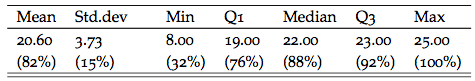
\includegraphics[width=0.65\textwidth]{image1a.png}}
\captionof{figure}{Summary statistics of student scores. The mean score was 82\% with a standard deviation of 15\%. Half of the students performed fairly well with a score of at least 88\%. However, there were low-scoring students, as the bottom quartile of students scored between 32\% and 76\% on this assignment.}
\label{fig:image1a}
\end{center}

In addition to understanding how students from this section performed overall for this topic, instructors and course coordinators may wish to determine how students performed across the different learning outcomes. Indeed, the report provides a fluctuation diagram for this purporse, see Figure \ref{fig:image1b}.

\begin{center}
\fbox{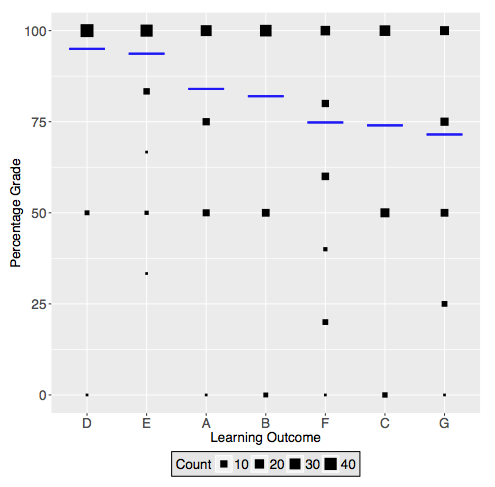
\includegraphics[width=0.75\textwidth]{image1b.png}}
\captionsetup{width=0.75\textwidth}
\captionof{figure}{Fluctuation diagram of percentage correct by learning outcome. The area of each square corresponds to the number of students who obtained that score for that learning outcome. Learning outcomes are ordered on the horizontal axis by mean score, with the highest mean score positioned on the left side of the axis. The mean score for each learning outcome is represented with a blue horizontal line. For this section, learning outcome \texttt{D} had the highest mean score, and learning outcome \texttt{G} had the lowest mean score. For each learning outcome, there remained a sizeable proportion of the 50 students who scored poorly (a score of at most 50\%).}
\label{fig:image1b}
\end{center}

Additionally, instructors and course coordinators may wish to obtain an overview of how students from this section performed across the different question sets within the learning outcomes. The report does generate such a graphic, which is shown in Figure \ref{fig:image1c}. 

\begin{center}
\captionsetup{width=0.65\textwidth}
\fbox{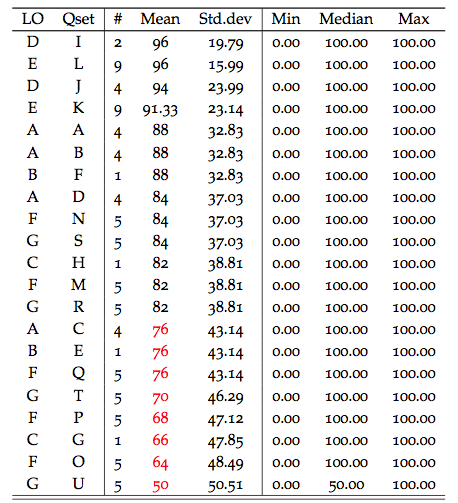
\includegraphics[width=0.65\textwidth]{image1c.png}}
\captionof{figure}{Summary statistics of the question sets. Rows are sorted by descending mean scores, which are marked red if less than 80\%. We see that there were eight question sets for which students of this section had a mean score of less than 80\%. Question Set \texttt{U} proved particularly difficult for this section of students, with a mean score of 50\%. }
\label{fig:image1c}
\end{center}

An instructor may wish to know which students from this section are performing poorly overall on this assignment. To assist this need, the report also includes a list of student names and their corresponding scores, for all cases of students who received a score below 80\% on the assignment, as is demonstrated in Figure \ref{fig:image1d}.

\begin{center}
\captionsetup{width=0.85\textwidth}
\fbox{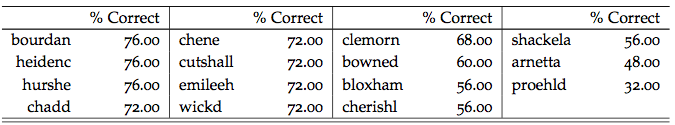
\includegraphics[width=0.85\textwidth]{image1d.png}}
\captionof{figure}{Of the 50 students in this section, 15 of them scored less than 80\% on this assignment.}
\label{fig:image1d}
\end{center}

\subsubsection{Contacts of low-performing students}
\label{sec:lowPerform}

Along the same lines, the report automatically generates a .txt file that lists the e-mails of all students who scored below 80\% on this assignment. The list is repeated, once in a comma-separated format, and once in a semicolon-separated format. These list formats are intended to provide instructors with a streamlined method to contact students, if needed, to inform them of their low-scoring performance and possibly to recommend seeking additional support and resources to improve their performance in future assignments. You can open the example .txt file we created in this vignette; it should be located in the \texttt{OutputFiles} subdirectory of the \texttt{extdata} example directory as (\texttt{Stat101hwk\_Topic06\_A\_lowScore.txt}).

What an instructor deems an approporiate threshold for a poor performance on a given assignment is arbitrary. For that reason, even though the default value of this threshold is 80, this threshold value can be altered by the user. Discussion and examples of how to alter certain default values in the \texttt{ePort} package, including the one just discussed, will occur later in the vignette in the section called \hyperref[sec:repOptions]{Report defaults}.

\subsection{One topic for one section - long version}

An instructor may be motivated to generate a long report for one topic and one section if they are seeking answers to the following types of questions:

\begin{enumerate}
\item \textit{Based on how students from this section performed on this topic, are there any noticeable problems where questions in certain question sets not being equally difficult?}
\item \textit{Which students from this section scored poorly on each learning outcome for this homework assignment?}
\item \textit{For each question in the assignment (particularly the difficult ones), what was the distribution of student responses?}
\end{enumerate}

\subsubsection{Code}

The short report we created for one section one topic (\texttt{Stat101hwk\_Topic06\_A-short.pdf}) may be helpful for users who want to view a brief and overall summarization of student performance. However, we can also generate a more verbose report summarization for one section one topic that would include additional details, such as a separate analysis for each problem in the assignment. We have already defined our three input file pathways and one output file pathway. Hence, if we wish to generate this longer version of the report summarization for one section one topic (sticking with section \texttt{A} and \texttt{Topic 06}), then all we need to rerun is the \texttt{makeReport()} function, only this time specifying the \texttt{reportType} parameter with the value of ``secTopicLong". \\

\begin{knitrout}
\definecolor{shadecolor}{rgb}{0.969, 0.969, 0.969}\color{fgcolor}\begin{kframe}
\begin{alltt}
\hlkwd{makeReport}\hlstd{(}\hlkwc{keyFile} \hlstd{= keyPath,} \hlkwc{dataFile} \hlstd{= dataPath,} \hlkwc{loFile} \hlstd{= loPath,} \hlkwc{outFile} \hlstd{=}
  \hlstd{outPath,} \hlkwc{reportType} \hlstd{=} \hlstr{"secTopicLong"}\hlstd{)}
\end{alltt}
\end{kframe}
\end{knitrout}

We can find our output report in the \texttt{OutputFiles} subdirectory of the \texttt{extdata} example directory. Indeed, we see that we now have a much longer report, called \texttt{Stat101hwk\_Topic06\_A-long.pdf}.

\subsubsection{Output}

The short report featured tools that identified individual students from the section who performed poorly overall. The long report provides a more detailed output that informs instructors on how each individual student did not only overall, but also for each learning outcome. This is shown below in Figure \ref{fig:image2a}.

\begin{center}
\captionsetup{width=0.75\textwidth}
\fbox{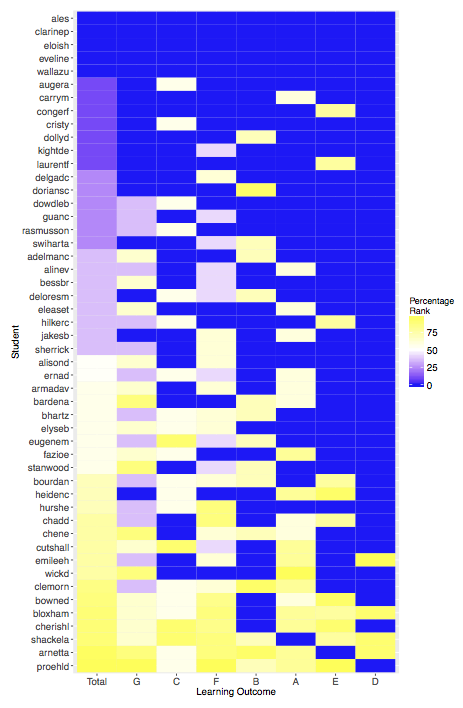
\includegraphics[width=0.75\textwidth]{image2a.png}}
\captionof{figure}{Heat map of the student ranks. Blue represents the top ranks, while yellow represents the bottom ranks. The order of students on the vertical axis is by overall rank across all learning outcomes. We see that the five students with the highest overall scores (ales, clarinep, eloish, eveline, and wallazu) performed well across all learning outcomes. Moreover, we see that the student with the lowest overall score (proehld) performed poorly for all learning outcomes, except for learning outcome \texttt{D}.}
\label{fig:image2a}
\end{center}

Oftentimes, one of the aims in an online homework assignment is to ensure that any two students in the course are not likely to receive the exact same set of questions on any given assignment, thereby encouraging students to complete their own work. However, it is important to ensure that all possible combinations of question subsets that a student could receive are equally difficult. Hence, it is necessary to confirm that all questions that can be randomly selected from each given question set are equally difficult. The long report does indicate this information to users, as is seen below in Figure \ref{fig:image2b}. Please note that this image is abridged for demonstration purposes; if you were to view the same image in the long report you just generated, then you would see that indeed it is a comprehensive table that consecutely lists the pertinent information for all 89 questions in this assignment. 

\begin{center}
\captionsetup{width=\textwidth}
\fbox{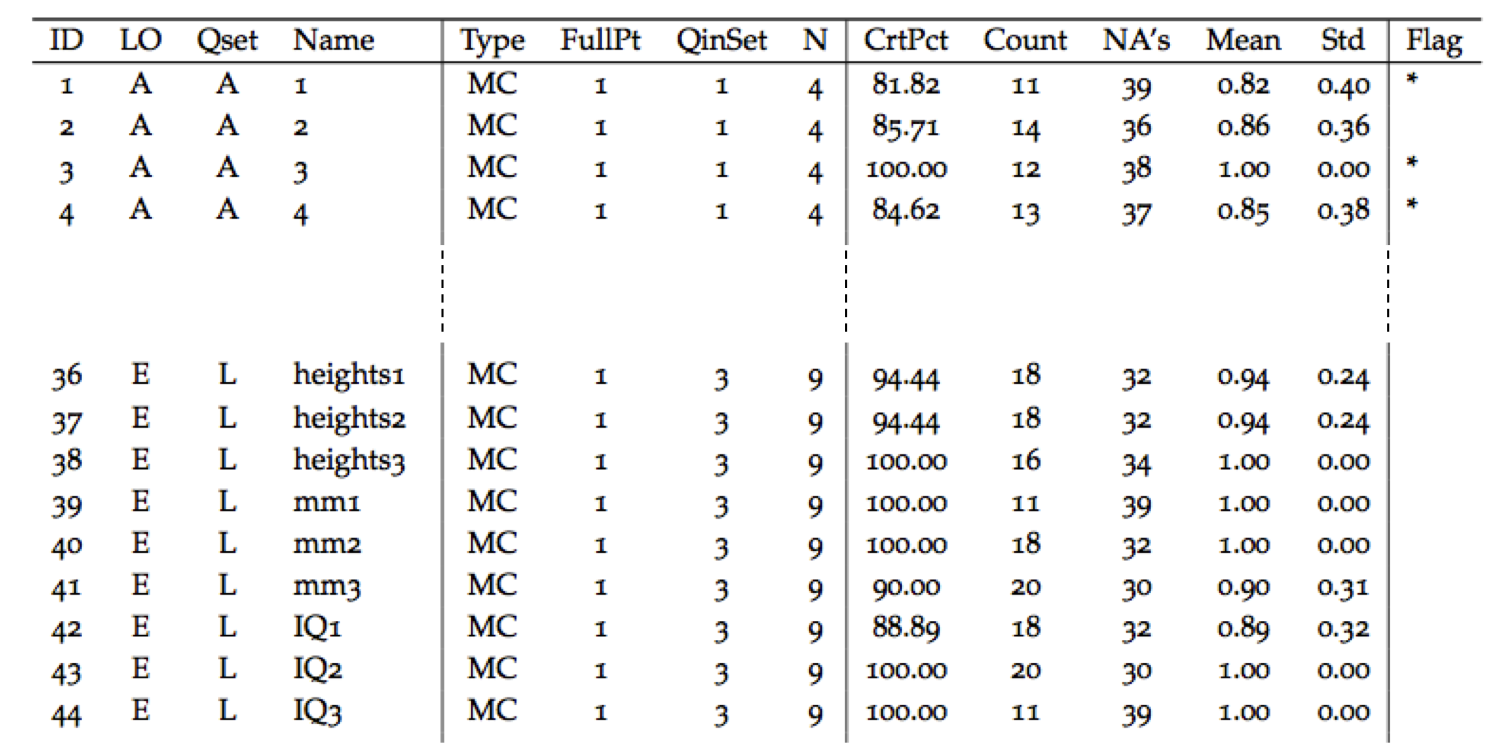
\includegraphics[width=\textwidth]{image2b.png}}
\captionof{figure}{Comparison of student performance in this section on each of the 89 possible questions of \texttt{Topic 06}, grouped by question set. If any pair of questions in a given question set have a difference in mean scores of more than 15\%, then both questions are flagged. Question set \texttt{A} contained four questions, with mean scores that ranged from 81.82\% to 100.00\%. Three of these questions (IDs: 1, 3, and 4) were flagged as having a mean score that was at least 15\% different than the mean score of at least one other question in this same question set. In contrast, question set \texttt{L} contained nine questions, with mean scores that ranged from 88.89\% to 100.00\%. Hence, none of these nine questions were flagged as demonstrating a concerningly large difference of at least 15\% in difficulty level from within the same question set.}
\label{fig:image2b}
\end{center}

As per the figure above, an instructor can quickly determine if there are questions for which students tend to show poor performance, and if there are question sets for which students tend to show disparate performance between their comprising questions. In either situation, an instructor may wish to examine these questions more closely, and determine how students are answering these questions incorrectly. For this reason, the long report also includes a summary of student responses for each individual question in the assignment, allowing instructors to determine the most common mistakes students in this section are making for these difficult questions.

If you open the long report we generated (\texttt{Stat101hwk\_Topic06\_A-long.pdf}), then you can view the summary for each of the 89 questions in this assignment. Each question has its summary printed on a separate page, beginning on Page 13 and ending on Page 101 of the report. As we saw in Figure \ref{fig:image2b}, the first Question ID of the assignment had a mean score of 81.82\%. We can ascertain what types of errors students from this section made on this Question ID by viewing its summary (on Page 13 of the report), which is provided below in Figure \ref{fig:image2c}. 

\begin{center}
\captionsetup{width=\textwidth}
\fbox{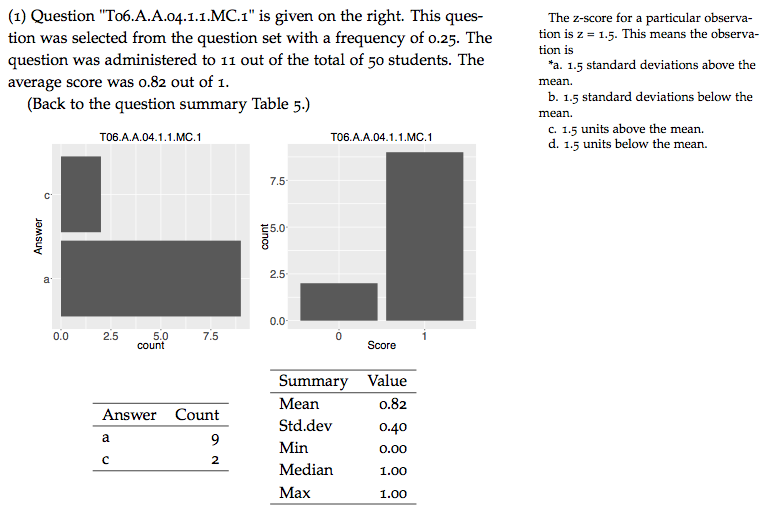
\includegraphics[width=\textwidth]{image2c.png}}
\captionof{figure}{A detailed summary of student performance for the first Question ID in the assignment. We see that 11 of the 50 students from this section received this question at random out of a question set that contains four similar questions. All 11 students responded with an answer: Nine correctly selected answer choice \texttt{A}, and two incorrectly selected answer choice \texttt{C}. No student incorrectly responded with answer choice \texttt{B} or \texttt{D}.}
\label{fig:image2c}
\end{center}

\subsection{One topic comparing multiple sections - short version}

An instructor may be motivated to generate a short report for one topic across multiple sections if they are seeking answers to the following types of questions:

\begin{enumerate}
\item \textit{For this topic, is there consistency across the sections in terms of overall performance?}
\item \textit{Combining students from all sections, are there any disparities in student performance between questions from the same question set of this topic?}
\item \textit{Combining students from all sections, are there any problematic questions in this topic, in which students typically perform poorly?}
\end{enumerate}

\subsubsection{Code}

Now that we know how to successfully generated reports for the three sections (\texttt{A}, \texttt{B}, and \texttt{C}) of \texttt{Topic 06} separately, we may wish to generate a report that compares the performance between these three sections. In this case, we use the same \texttt{makeReport()} function, just as we did before. However, for our parameter \texttt{dataFile}, we will input a list \texttt{dataList} that contains the paths to the data files for both sections we wish to compare. Of course, we must also correctly specify the \texttt{reportType} parameter to indicate that we wish to generate a short report that compares sections for a given topic: \\

\begin{knitrout}
\definecolor{shadecolor}{rgb}{0.969, 0.969, 0.969}\color{fgcolor}\begin{kframe}
\begin{alltt}
\hlstd{dataFolder} \hlkwb{=} \hlkwd{system.file}\hlstd{(}\hlstr{"inst/extdata/DataFiles/Topic06"}\hlstd{,} \hlkwc{package} \hlstd{=} \hlstr{"ePort"}\hlstd{)}
\hlstd{dataList} \hlkwb{=} \hlkwd{list.files}\hlstd{(}\hlkwc{path} \hlstd{= dataFolder,} \hlkwc{full.names} \hlstd{=} \hlnum{TRUE}\hlstd{)[}\hlnum{1}\hlopt{:}\hlnum{3}\hlstd{]}
\hlkwd{makeReport}\hlstd{(}\hlkwc{keyFile} \hlstd{= keyPath,} \hlkwc{dataFile} \hlstd{= dataList,} \hlkwc{loFile} \hlstd{= loPath,} \hlkwc{outFile} \hlstd{=}
  \hlstd{outPath,} \hlkwc{reportType} \hlstd{=} \hlstr{"crossSecTopicShort"}\hlstd{)}
\end{alltt}
\end{kframe}
\end{knitrout}

Please ensure that the variable \texttt{dataList} contains exactly the full pathway to the three data files (\texttt{Topic06.A.csv}, \texttt{Topic06.B.csv}, and \texttt{Topic06.C.csv}). If your variable contains additional pathways, then you have more than just the three necessary input data files in your \texttt{DataFiles/Topic06} folder. If that is the case, then you will need to move these extraneous files elsewhere or hardcode the three full pathways into the \texttt{dataList} variable. 

\subsubsection{Output}

You should be able to examine the report we just generated (\texttt{Stat101hwk\_Topic06\_crossSection\-short.pdf}) in our example \texttt{OutputFiles} folder. A course coordinator may wish to know if student performance for learning outcomes is similar across sections. In the report we just produced, we can indeed quickly obtain this information, as is shown below in Figure \ref{fig:image3a}.

\begin{center}
\captionsetup{width=0.6\textwidth}
\fbox{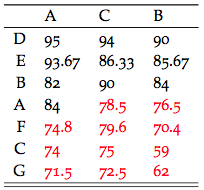
\includegraphics[width=0.3\textwidth]{image3a.png}}
\captionof{figure}{Average percentages correct for each learning outcome by section. Learning outcomes are sorted by the average percentages correct across all sections, from the highest to the lowest. Scores in red represent cases where a section had an average score for a learning outcome that was less than 80\%. We see that the sections showed consistency in that they all did well for learning outcomes \texttt{D}, \texttt{E}, and \texttt{B}, and all did poorly for learning outcomes \texttt{F}, \texttt{C}, and \texttt{G}.}
\label{fig:image3a}
\end{center}

The report also provides tables that, after combining student responses from all sections, displays questions that have a low overall performance score. It additionally includes tables that highlight question sets that seem to have disparate performance scores between the questions from which they are composed.

\subsection{One topic comparing multiple sections - long version}

An instructor may be motivated to generate a long report for one topic across multiple sections if they are seeking answers to the following types of questions:

\begin{enumerate}
\item \textit{For this topic, is there consistency across the sections in terms of overall performance, and in terms of performance by learning outcome and question set?}
\item \textit{Combining students from all sections, for this topic, are there any disparities in student performance between questions from the same question set?}
\item \textit{Combining students from all sections, for this topic, are there any learning outcomes or question sets for which students consistently tend to perform poorly?}
\item \textit{Combining students from all sections, for this topic, for each question in the assignment (particularly the difficult ones), what was the distribution of student responses?}
\end{enumerate}

\subsubsection{Code}

We received a brief comparative summary between the three sections for \texttt{Topic 06} in the previous section of this vignette. If we would like to see a more detailed version of this report that includes comparative information for each question in the topic of interest, then we can simply run the previous line of code, only now specifying the \texttt{reportType} parameter to indicate that we wish to generate a long report that compares sections for a given topic: \\

\begin{knitrout}
\definecolor{shadecolor}{rgb}{0.969, 0.969, 0.969}\color{fgcolor}\begin{kframe}
\begin{alltt}
\hlkwd{makeReport}\hlstd{(}\hlkwc{keyFile} \hlstd{= keyPath,} \hlkwc{dataFile} \hlstd{= dataList,} \hlkwc{loFile} \hlstd{= loPath,} \hlkwc{outFile} \hlstd{=}
  \hlstd{outPath,} \hlkwc{reportType} \hlstd{=} \hlstr{"crossSecTopicLong"}\hlstd{)}
\end{alltt}
\end{kframe}
\end{knitrout}

\subsubsection{Output}

The code above should have generated the long edition of the report (\texttt{Stat101hwk\_Topic06\_crossSection\-long.pdf}). One of the most immediate pieces of information that a course coordinator may wish to glean is whether or not there are discrepancies in student performance for a given topic across multiple sections. This could be especially true if there are different instructors and/or different teaching methods being employed across the different sections. In the report we just produced, we can indeed quickly compare how the students performed overall for \texttt{Topic 06} across the three sections in a table that has been copied here in Figure \ref{fig:image4a}.

\begin{center}
\captionsetup{width=0.7\textwidth}
\fbox{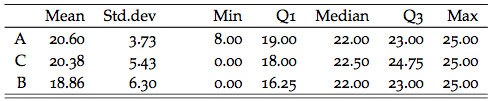
\includegraphics[width=0.7\textwidth]{image4a.png}}
\captionof{figure}{The mean, standard deviation, and five number summary for student performance across the three sections. We see that the overall student performance was relatively similar across the three sections, although sections \texttt{A} and \texttt{C} had overall mean scores that were at least 1.5 points larger than the overall mean score of section \texttt{B}.}
\label{fig:image4a}
\end{center}

While the short report allowed us to compare how students performed in \texttt{Topic 06} across the sections, the long report will also allow us to make comparisons of student performance across the sections at a more detailed level of learning outcomes and question sets. For instance, the long report includes comparative information at the level of learning outcomes, as is illustrated in Figure \ref{fig:image4b}.

\begin{center}
\captionsetup{width=0.8\textwidth}
\fbox{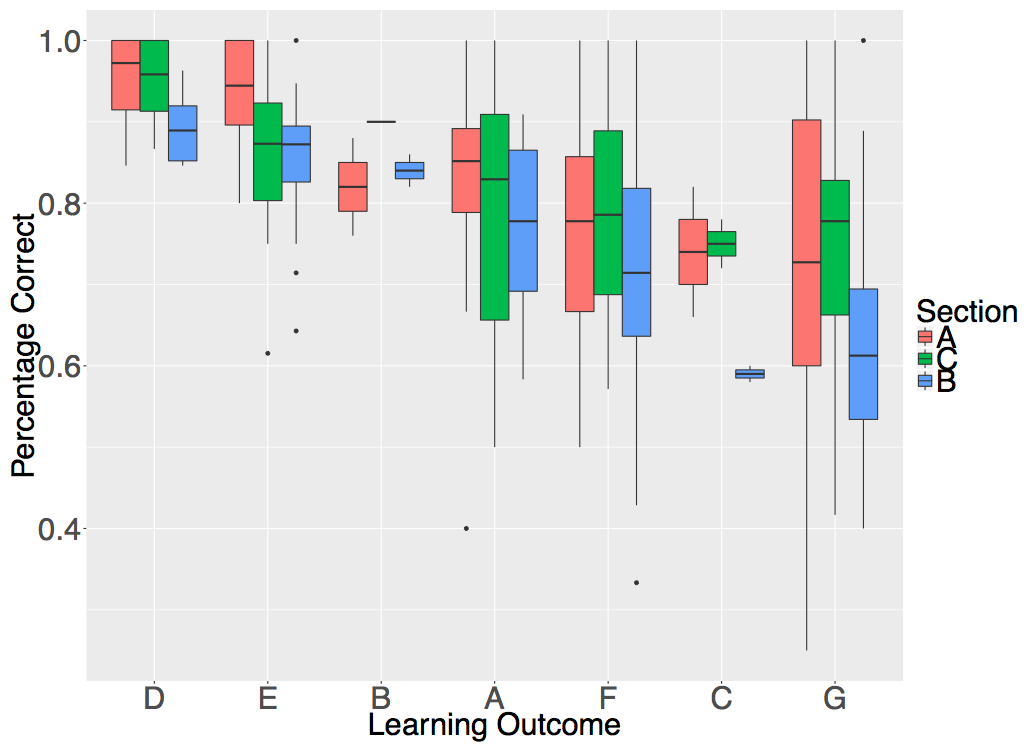
\includegraphics[width=0.8\textwidth]{image4b.png}}
\captionof{figure}{The three sections were fairly comparable in their performances across the learning outcomes. In general, learning outcomes (such as \texttt{B}) that showed little variance between students in a given section also showed little variance between students in the other sections, while some learning outcomes (such as \texttt{G}) that showed large variance between students in a given section also showed large variance between students in the other sections. Notably, for learning outcome \texttt{C}, all students in section \texttt{B} performed less well than all students from sections \texttt{A} and \texttt{C}; likewise, for learning outcome \texttt{B}, all students in section \texttt{C} outperformed all students from sections \texttt{A} and \texttt{B}.}
\label{fig:image4b}
\end{center}

The long edition of the report breaks it down further by comparing the three sections at the level of each question set. This is demonstrated below in Figure \ref{fig:image4c}.

\begin{center}
\captionsetup{width=0.55\textwidth}
\fbox{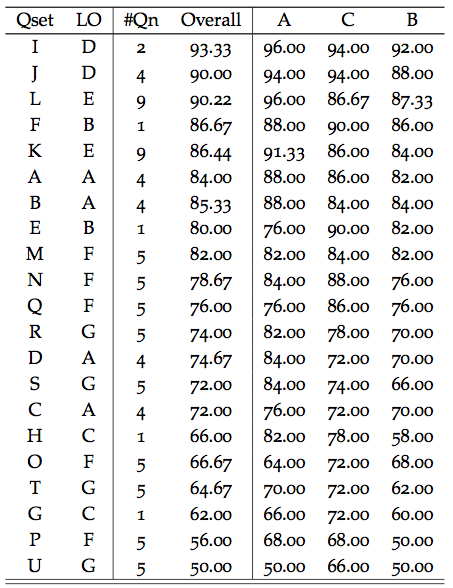
\includegraphics[width=0.55\textwidth]{image4c.png}}
\captionof{figure}{Mean percent scores for each question set by section. The question sets are sorted by decreasing overall mean scores. Both question sets with the highest overall mean scores across sections are from learning outcome \texttt{D}. We see that sections performed fairly consistently across question sets. However, question set \texttt{H} had a mean score difference of 24\% between sections \texttt{A} and \texttt{B}.}
\label{fig:image4c}
\end{center}

The long edition of the report also offers tools that do not explicitly compare the sections of interest, but instead, combine data from all the sections of interest to generate more power in any analysis that we could instead do separately using just the data from one section. For instance, we previously demonstrated certain tools in the individual section reports that can allow instructors to confirm that their students will receive equally-challenging randomly-selected subsets of questions; this was shown in Figure \ref{fig:image2b}.

A course coordinator could again explore this same potential predicament, only now using the data combined from students across both sections, as is displayed in Figure \ref{fig:image4d}. Please note that this image is abridged for demonstration purposes. If you were to view the same image in the long report you just generated, then you would see that indeed it is a comprehensive table that consecutely lists the pertinent information for all 89 possible questions in this assignment.

\begin{center}
\captionsetup{width=\textwidth}
\fbox{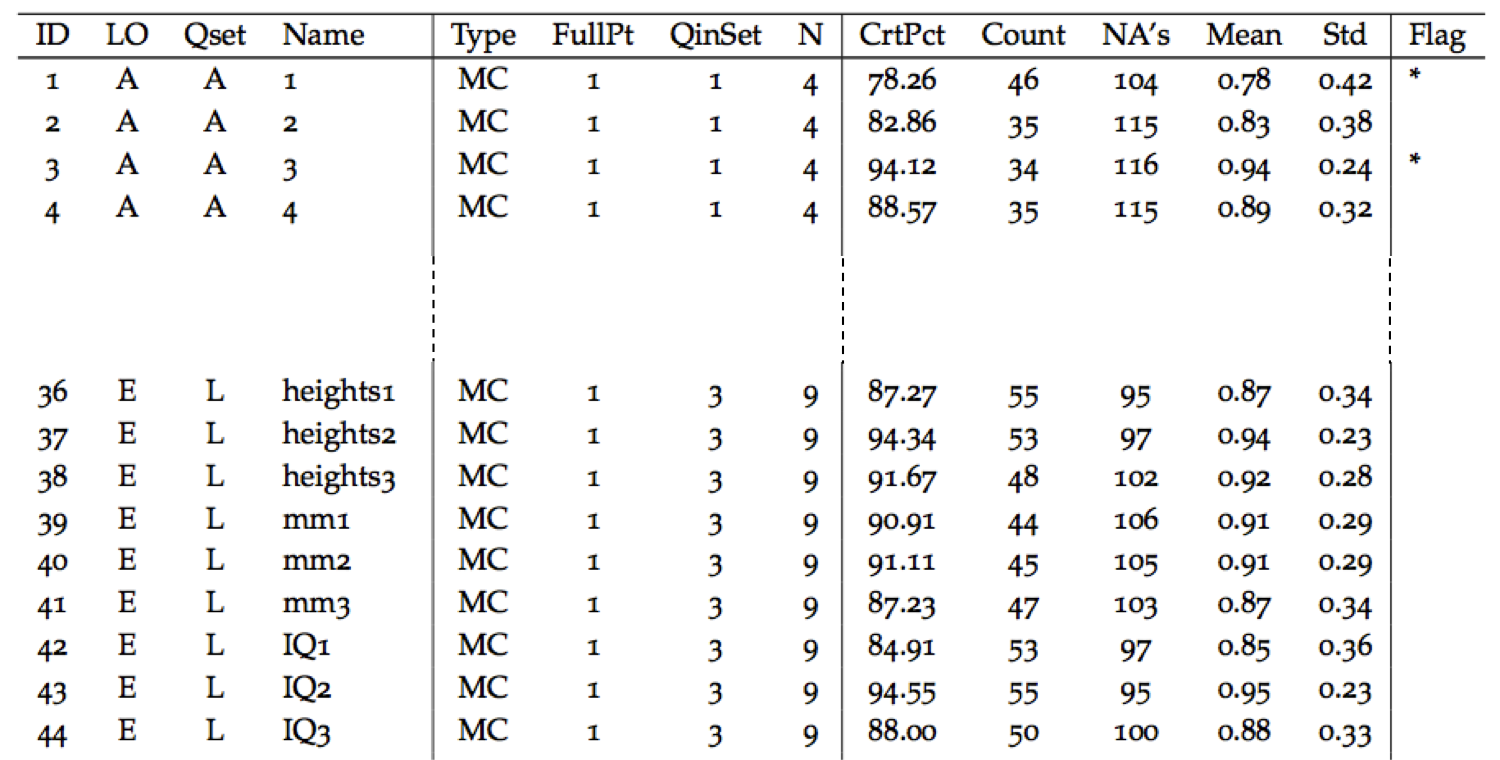
\includegraphics[width=\textwidth]{image4d.png}}
\captionof{figure}{Combined student performance from sections \texttt{A}, \texttt{B}, and \texttt{C} on each question of \texttt{Topic 06}, grouped by question set. If any pair of questions in a given question set have a difference in mean scores of more than 15\%, then both questions are flagged. Question set \texttt{A} contained four problems, and when we only used student performance information from the 50 students in section \texttt{A}, three IDs (1, 3, and 4) were flagged as having a mean score that was at least 15\% different than the mean score of another question in the same question set (see Figure \ref{fig:image2b}). However, now that we have combined student performance information from all 150 students across the three sections, only two IDs (1 and 3) remain flagged. In contrast, question set \texttt{I} contained nine problems, and none of these problems were flagged first when we only used the 50 student performances in section \texttt{A} (see Figure \ref{fig:image2b}) and now when we use all 150 student performances across the three sections.}
\label{fig:image4d}
\end{center}

As per the figure above, an instructor can quickly determine if there are questions for which students tend to perform poorly, and if there question sets for which students tend to show inconsistent performance between the individual questions. In either situation, an instructor may wish to examine these questions more closely, and determine how students are answering these problems incorrectly. For this reason, the long report also includes a summary of student responses for each individual problem in the assignment, allowing instructors to determine the most common mistakes students across the sections are making for these difficult questions.

If you open the long report we generated (\texttt{Stat101hwk\_Topic06\_crossSection-long.pdf}), then you can view the summary for each of the 89 possible questions in this assignment. Each question summary is printed on a separate page, beginning on Page 11 and ending on Page 100 of the report. As we saw in Figure \ref{fig:image4d}, Question ID 1 had an overall mean score of 78.26\% across the three sections. We can ascertain what types of errors students made on this problem, regardless of section, by viewing the summary for Question ID 1 (on Page 11 of the report), which is provided below in Figure \ref{fig:image4e}. Of course, now that we are collecting student responses from the 46 students who received this problem in any of the three sections, we are provided with more power about the distribution of student responses than when only considered the 11 students in section \texttt{A}, as was done in Figure \ref{fig:image2c}.

\begin{center}
\captionsetup{width=\textwidth}
\fbox{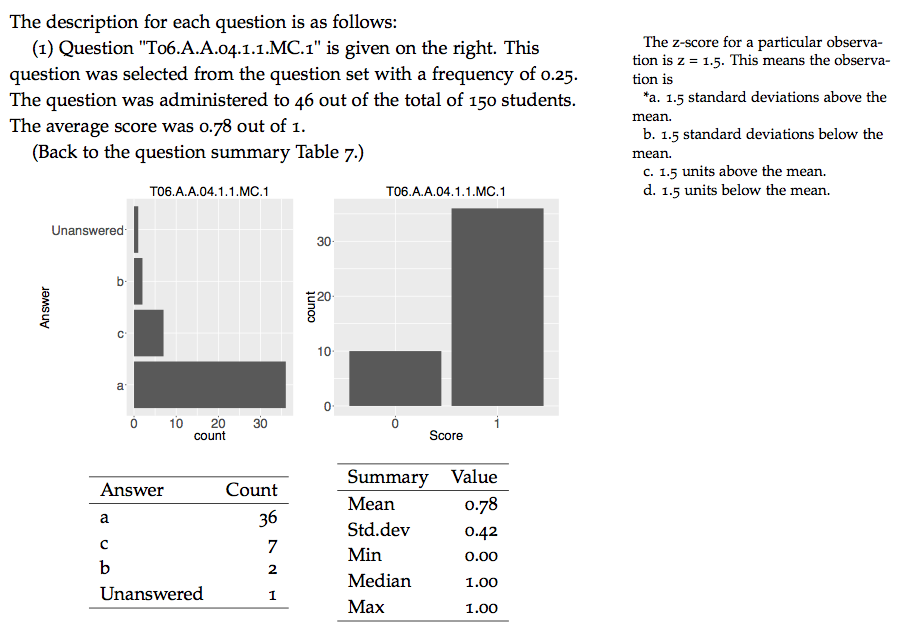
\includegraphics[width=\textwidth]{image4e.png}}
\captionof{figure}{A detailed summary of student performance for the first Question ID in the assignment. Of the 46 students who received this Question ID,  36 students correctly selected answer choice \texttt{A}. The most frequently incorrect response from students was answer choice \texttt{C}, followed by answer choice \texttt{B}. No students incorrectly answered choice \texttt{D}. One student did not respond. In general, this is a similar distribution to what we saw in Figure \ref{fig:image2c}, when we only examined the 11 students from section \texttt{A} who received this Question ID.}
\label{fig:image4e}
\end{center}

\subsection{One unit (group of topics) for one section}

An instructor may be motivated to generate a long report for one unit (group of topics) and one section if they are seeking answers to the following types of questions:

\begin{enumerate}
\item \textit{Did the students from this section overall perform comparably between the topics of interest?}
\item \textit{Are there are any patterns in how individual students from this section performed between the topics of interest?}
\item \textit{How often are the students from this section missing assignments? Are there any topics for which students from this section in particular miss assignments?}
\end{enumerate}

\subsubsection{Code}

To generate this type of report, we must be sure to provide a \texttt{dataFolder} variable that contains the pathway to a folder that contains our data files of interest. As usual, it is important to ensure that there are no extraneous files in our folder. Since we want to examine three sections (\texttt{A}, \texttt{B}, and \texttt{C}) and three topics (\texttt{06}, \texttt{07}, and \texttt{08}), then we need a folder that contains nothing other than the data files for the nine possible combinations of these sections and topics.

Indeed, the \texttt{ePort} package contains such an example folder, which he have not yet used in this vignette. It is located in \texttt{extdata/DataFiles/Topic06\_07\_08}. You can examine this folder to confirm that there is nothing but our nine necessary input files (\texttt{Topic06.A.csv}, \texttt{Topic06.B.csv}, \texttt{Topic06.C.csv}, \texttt{Topic07.A.csv}, \texttt{Topic07.B.csv}, \texttt{Topic07.C.csv}, \texttt{Topic08.A.csv}, \texttt{Topic08.B.csv}, and \texttt{Topic08.C.csv}). We save the pathway to all nine of these files to a variable called \texttt{dataList}.

For this type of report, we must also prepare a few variables before running the \texttt{makeReport()} function. We prepare these variables using the \texttt{setDir()}, \texttt{mergeData()}, and \texttt{subsetData()} functions. For more information about these functions, please use the \texttt{help()} command. The \texttt{dataTable} variable we create below is a simple data frame that specifies the topic and section for each input data file of interest. The \texttt{mergedData} variable we also create below is a list of data frames that contains the scores that each student from the three sections earned on each topic assignment, the number of missed assignments, and the total scores across all students for each section and topic.

Our goal here is to create a separate report for each section of interest, where each report compares how students from that section performed across topics. We can most efficiently accomplish this by using a for loop, as shown below, where we create one last variable \texttt{merged}. This variable is the subset of our \texttt{mergedData} variable that only applies for the section of interest.

Lastly, we can run our \texttt{makeReport()} function on this section and group of topics. We should specify our unit variable, which contains a default value of 1. In our example, we are indicating that we consider topics \texttt{06}, \texttt{07}, and \texttt{08} to be from \texttt{Unit 2}.\\

\begin{knitrout}
\definecolor{shadecolor}{rgb}{0.969, 0.969, 0.969}\color{fgcolor}\begin{kframe}
\begin{alltt}
\hlstd{dataFolder} \hlkwb{=} \hlkwd{system.file}\hlstd{(}\hlstr{"inst/extdata/DataFiles/Topic06_07_08"}\hlstd{,} \hlkwc{package}\hlstd{=}\hlstr{"ePort"}\hlstd{)}
\hlstd{dataList} \hlkwb{=} \hlkwd{list.files}\hlstd{(}\hlkwc{path} \hlstd{= dataFolder,} \hlkwc{full.names} \hlstd{=} \hlnum{TRUE}\hlstd{)}

\hlkwa{for} \hlstd{(file} \hlkwa{in} \hlstd{dataList)\{}
  \hlkwd{rewriteData}\hlstd{(file)}
\hlstd{\}}

\hlstd{dataTable} \hlkwb{=} \hlkwd{setDir}\hlstd{(dataFolder)}
\hlstd{mergedData} \hlkwb{=} \hlkwd{mergeData}\hlstd{(dataTable)}

\hlkwa{for} \hlstd{(section} \hlkwa{in} \hlkwd{unique}\hlstd{(dataTable}\hlopt{$}\hlstd{section))\{}
  \hlstd{merged} \hlkwb{=} \hlkwd{subsetData}\hlstd{(mergedData, dataTable,} \hlkwc{choice} \hlstd{= section)}
  \hlkwd{makeReport}\hlstd{(}\hlkwc{outFile} \hlstd{= outPath,} \hlkwc{unit} \hlstd{=} \hlnum{2}\hlstd{,} \hlkwc{section} \hlstd{= section,} \hlkwc{reportType} \hlstd{=} \hlstr{"secUnit"}\hlstd{)}
\hlstd{\}}
\end{alltt}
\end{kframe}
\end{knitrout}

Upon running this code, you should have created three files into your \texttt{OutputFiles} folder, \texttt{Stat101hwk\_Unit2\_A.pdf}, \texttt{Stat101hwk\_Unit2\_B.pdf}, and \texttt{Stat101hwk\_Unit2\_C.pdf}. Each of these files compares how students in that section performed for the three topics that we defined as comprising \texttt{Unit 2}.

\subsubsection{Output}

An instructor might want to know how his or her section of students is performing throughout the course duration, and in partiular, if there are any topics within a unit of interest for which their students perform well or poorly. We will examine one of the three reports we just generated (\texttt{Stat101hwk\_Unit2\_A.pdf}) to discover the types of tools that instructors could use in such situations. The report begins with a quick summary of how students performed for this section (\texttt{A}) across all topics in \texttt{Unit 2} (topics \texttt{06}, \texttt{07}, and \texttt{08}), as is provided in Figure \ref{fig:image5a}.

\begin{center}
\captionsetup{width=0.65\textwidth}
\fbox{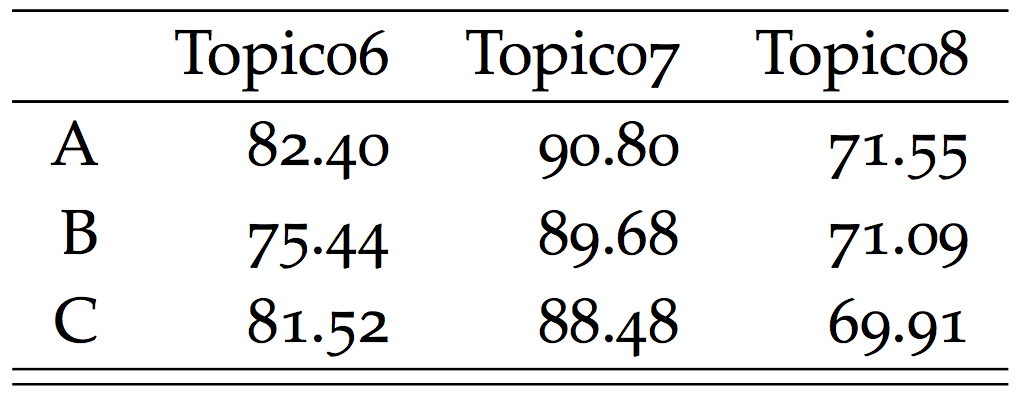
\includegraphics[width=0.65\textwidth]{image5a.png}}
\captionof{figure}{Overall summary of how students in section \texttt{A} performed for topics \texttt{06}, \texttt{07}, and \texttt{08}. Students showed the highest mean and median for \texttt{Topic 07}, and the lowest mean and median for \texttt{Topic 08}.}
\label{fig:image5a}
\end{center}

We can also compare how this section of students performed between these three topics, not only at an overall level, but also at the individual student level, see Figure \ref{fig:image5b}.

\begin{center}
\captionsetup{width=0.65\textwidth}
\fbox{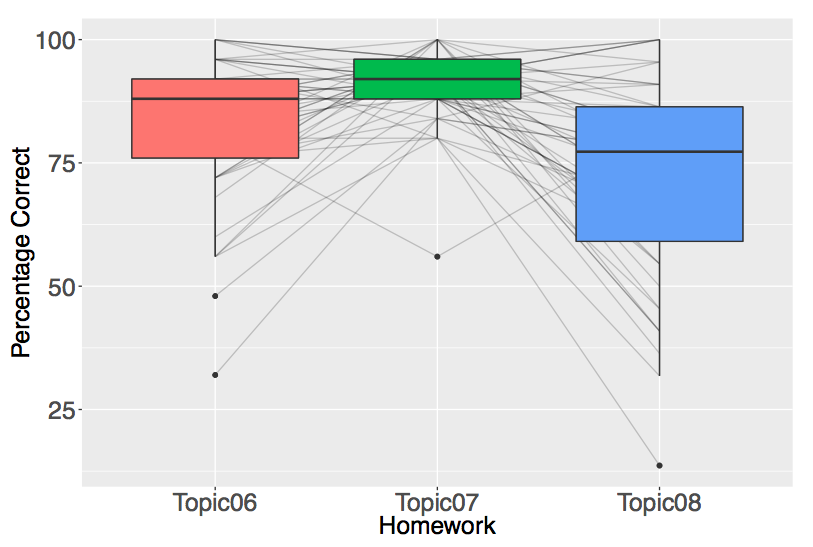
\includegraphics[width=0.65\textwidth]{image5b.png}}
\captionof{figure}{Boxplots with parallel coordinate plot overlaid. Each boxplot represents the distribution of all student scores for a given topic, and each parallel coordinate line represents the scores across all topics for a given student. We see that how a given student performed relative to the rest of the students was, in most cases, consistent across the three topics.}
\label{fig:image5b}
\end{center}

While the figure above can allow us to see if there are trends in how individual students scored between the topics, if we find patterns of interest, we may wish to determine the identity of individual students. This is provided below in Figure \ref{fig:image5c}.

\begin{center}
\captionsetup{width=0.65\textwidth}
\fbox{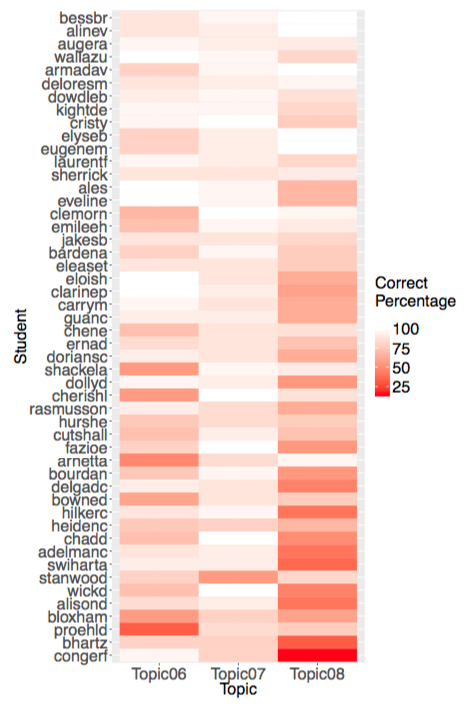
\includegraphics[width=0.65\textwidth]{image5c.png}}
\captionof{figure}{Heat map of the student scores in this section for the three topics of interest. The students are listed in descending order of their overall average score across the three sections. We can determine that the lowest-performing student (congerf) performed much worse as the topics progressed. In contrast, the highest-performing student (bessbr) performed slightly better as the topics progressed.}
\label{fig:image5c}
\end{center}

The report also produces tables that provide information about missed assignments for this section of students. An instructor could use this tool to determine if there are certain topics for which students from the section of interest tend to fail to submit the assignment, or if there are certain students from this section who tend to fail to submit assignments regardless of topic.

\subsection{One unit (group of topics) comparing multiple sections}

An instructor may be motivated to generate a report for multiple topics and multiple sections if they are seeking answers to the following types of questions:

\begin{enumerate}
\item \textit{Are there certain sections that either perform better or worse consistently across topics?}
\item \textit{What are the easiest and most difficult topics in the course, regardless of section?}
\item \textit{Are there any patterns in missed assignments by section or by topic?}
\end{enumerate}

\subsubsection{Code}
\label{sec:crossSecU}

To accomplish this task, we create a \texttt{merged} variable that contains a list of data frames that include the raw scores, percentage scores, number of missing assignments, and average scores for the three sections and three topics of interest. After that, we can simply use our \texttt{makeReport()} command, being sure to specify that we are designating the three topics (\texttt{06}, \texttt{07}, and \texttt{08}) as \texttt{Unit 2}. \\

\begin{knitrout}
\definecolor{shadecolor}{rgb}{0.969, 0.969, 0.969}\color{fgcolor}\begin{kframe}
\begin{alltt}
\hlstd{merged} \hlkwb{=} \hlkwd{subsetData}\hlstd{(mergedData, dataTable)}
\hlkwd{makeReport}\hlstd{(}\hlkwc{outFile} \hlstd{= outPath,} \hlkwc{unit} \hlstd{=} \hlnum{2}\hlstd{,} \hlkwc{reportType} \hlstd{=} \hlstr{"crossSecUnit"}\hlstd{)}
\end{alltt}
\end{kframe}
\end{knitrout}

This creates four files, \texttt{Stat101hwk\_Unit2\_crossSection.pdf}, \texttt{Stat101hwk\_Unit2\_A\_lowScore.txt}, \texttt{Stat101hwk\_Unit2\_B\_lowScore.txt}, and \texttt{Stat101hwk\_Unit2\_C\_lowScore.txt}. The first file contains our report that compares all combinations of the three sections and three topics of interest. The latter three .txt files contain lists of the e-mail contacts of students from each respective section who performed poorly consistently across the three topics of interest.

\subsubsection{Output}

From the report we just generated (\texttt{Stat101hwk\_Unit2\_crossSection.pdf}), we can simultaneously examine how students performed across different sections and different topics. As is the case with previous reports, we are provided some basic summaries, as provided in Figure \ref{fig:image6a}.

\begin{center}
\captionsetup{width=0.4\textwidth}
\fbox{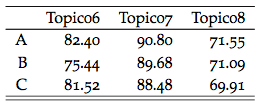
\includegraphics[width=0.4\textwidth]{image6a.png}}
\captionof{figure}{Mean scores for all sections and topics of interest. Section \texttt{A} had the highest mean score for all three topics.}
\label{fig:image6a}
\end{center}

In this report, we can also compare score distributions for each combination of section and topic (see Figure \ref{fig:image6b}).

\begin{center}
\captionsetup{width=0.8\textwidth}
\fbox{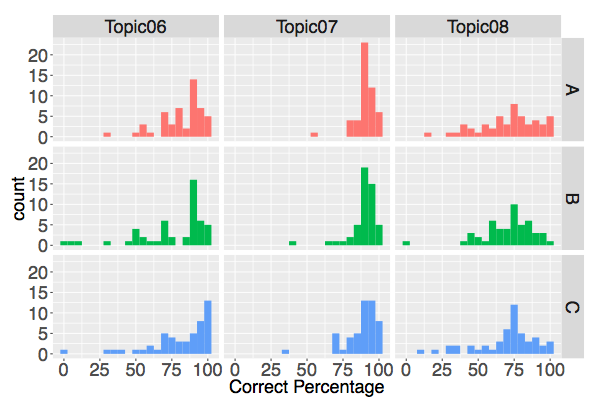
\includegraphics[width=0.8\textwidth]{image6b.png}}
\captionof{figure}{Histogram of student scores for the sections and topics of interest. We see that, for all sections, the score distribution for \texttt{Topic 08} appeared more uniform compared to the score distributions for topics \texttt{06} and \texttt{07}.}
\label{fig:image6b}
\end{center}

One other feature of this report is a tabulation of missing homework for sections and topics of interest (see Figure \ref{fig:image6c}). If there are patterns found for this, course coordinators may wish to determine what is causing students to tend to miss homework assignments for a certain section or certain topic.

\begin{center}
\captionsetup{width=0.75\textwidth}
\fbox{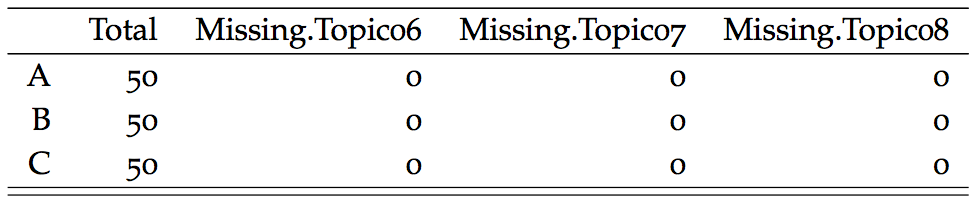
\includegraphics[width=0.75\textwidth]{image6c.png}}
\captionof{figure}{Missing homework summary for the three sections and three topics of interest. In each of the three sections, all fifty students submitted homework assignments for all three topics of interest.}
\label{fig:image6c}
\end{center}

\subsubsection{Contacts of low-performing students}
\label{sec:lowPer}

This report type automatically generates a .txt file for each section that lists the e-mail contacts of all students from that section who scored below a threshold of 20\% on at least half of the topic assignments. The format of these .txt files is similar to the one that we already generated for the \hyperref[sec:lowPerform]{short version of the report on one section and one topic}. We can alter this threshold, as will be described in a later section of the vignette (\hyperref[sec:repOptions]{Report defaults}).

You can take a moment to examine these three files (\texttt{Stat101hwk\_Unit2\_A\_lowScore.txt}, \texttt{Stat101hwk\_Unit2\_B\_lowScore.txt}, and \texttt{Stat101hwk\_Unit2\_C\_lowScore.txt}). If you do so, you will notice that Section \texttt{A} contained three low-performers, Section \texttt{B} contained two low-performers, and Section \texttt{C} contained six low-performers.

\section{Additional tools}

\subsection{Splitting files}

In some cases, one homework assignment may span across two topics. In order to generate separate reports for each of the two topics, we will first need to split the data file. In our example, we will split the Chapter 20 data files into Topics 21 and 22 reports for all three sections. We have a special folder in our example data to complete this process; if you examine the folder called \texttt{Chapter20\_Split}, which is located in our example \texttt{DataFiles} folder, then you will see that it contains the three files, \texttt{Chapter20.A.csv}, \texttt{Chapter20.B.csv}, and \texttt{Chapter20.C.csv}.

If you open any of these three files, then you will notice there is a ``Question ID" column and a ``Question" column (which contains Question RsQ). The Question ID refers to the order of the questions that each student received; in this example assignment, there are 17 Question IDs. Hence, each student received 17 questions, and should have Question IDs for each of these questions consecutively increasing from Question ID 1 to Question ID 17. In contrast, the Question RsQ refers to the absolute ID from \hyperref[sec:ResSection]{Respondus}. In this assignment, in total, there were 55 questions in \texttt{Respondus}, from which each student received their randomly-selected subset of 17 questions Hence, the Question RsQ should range from 1 to 55.

Because of this, if an instructor wants to split the data files, there are two parameters they can use to designate the cut location. If you run a \hyperref[sec:helpSection]{help()} function on the \texttt{ePort} function \texttt{splitFile()}, then you see that these cut types are called ``RsQ" and ``ID". Let us say that we need to split these data files into one file that only contains the first 7 ID Questions and another file that only contains the last 10 ID Questions. In that case, we can choose a cut type of ``ID" with a value of 7, which corresponds to a cut type of ``RsQ" with a value of 13. We show this process below using the cut type of ``ID". \\

\begin{knitrout}
\definecolor{shadecolor}{rgb}{0.969, 0.969, 0.969}\color{fgcolor}\begin{kframe}
\begin{alltt}
\hlstd{dataFolder} \hlkwb{=} \hlkwd{system.file}\hlstd{(}\hlstr{"inst/extdata/DataFiles/Chapter20_Split"}\hlstd{,} \hlkwc{package} \hlstd{=} \hlstr{"ePort"}\hlstd{)}
\hlstd{dataList} \hlkwb{=} \hlkwd{list.files}\hlstd{(}\hlkwc{path} \hlstd{= dataFolder,} \hlkwc{full.names} \hlstd{=} \hlnum{TRUE}\hlstd{)[}\hlnum{1}\hlopt{:}\hlnum{3}\hlstd{]}

\hlkwa{for}\hlstd{(file} \hlkwa{in} \hlstd{dataList)\{}
  \hlkwd{rewriteData}\hlstd{(file)}
  \hlkwd{splitFile}\hlstd{(file,} \hlnum{7}\hlstd{,} \hlstr{"ID"}\hlstd{)}
\hlstd{\}}
\end{alltt}
\end{kframe}
\end{knitrout}

Upon running the above code, if you return to the \texttt{Chapter20\_Split} folder, then you will see that six new files have been created, \texttt{Chapter20.A.part1.csv}, \texttt{Chapter20.A.part2.csv}, \texttt{Chapter20.B.part1.csv}, \texttt{Chapter20.B.part2.csv}, \texttt{Chapter20.C.part1.csv}, and \texttt{Chapter20.C.part2.csv}. You can verify that the \texttt{part1} files contain the first 7 Question IDs, while the \texttt{part2} files contain the last 10 Question IDs.

\subsection{Merging files}

In some cases, one topic might encompass two homework assignments. In order to generate a report for the overall topic, we will first need to combine the two data files. Such a scenario exists in the \hyperref[sec:OnlineHomework]{online database}, in which Chapter 9 and 12 homework assignments together form \texttt{Topic 11}.

In our example, we will combine the Chapter 9 and 12 homework assignments to form the \texttt{Topic 11} data file for sections \texttt{A}, \texttt{B}, and \texttt{C}. We again have a special folder in our example data to complete this process. It is located in our example \texttt{DataFiles} folder in a subfolder called \texttt{Topic11\_Merge}. Upon entering this folder, you should see that it contains six files, \texttt{Ch9.A.csv}, \texttt{Ch9.B.csv}, \texttt{Ch9.C.csv}, \texttt{Ch12.A.csv}, \texttt{Ch12.B.csv}, and \texttt{Ch12.C.csv}. Notice in the code below that we save the topic number to a string variable called \texttt{topicNum}. \\

\begin{knitrout}
\definecolor{shadecolor}{rgb}{0.969, 0.969, 0.969}\color{fgcolor}\begin{kframe}
\begin{alltt}
\hlstd{dataFolder} \hlkwb{=} \hlkwd{system.file}\hlstd{(}\hlstr{"inst/extdata/DataFiles/Topic11_Merge"}\hlstd{,} \hlkwc{package}\hlstd{=}\hlstr{"ePort"}\hlstd{)}
\hlstd{dataList} \hlkwb{=} \hlkwd{list.files}\hlstd{(}\hlkwc{path} \hlstd{= dataFolder,} \hlkwc{full.names}\hlstd{=}\hlnum{TRUE}\hlstd{)[}\hlnum{1}\hlopt{:}\hlnum{6}\hlstd{]}
\hlstd{topicNum} \hlkwb{=} \hlstr{"Topic11"}

\hlkwa{for} \hlstd{(i} \hlkwa{in} \hlstd{dataList)} \hlkwd{rewriteData}\hlstd{(i)}

\hlkwa{for}\hlstd{(i} \hlkwa{in} \hlkwd{c}\hlstd{(}\hlstr{'A'}\hlstd{,} \hlstr{'B'}\hlstd{,} \hlstr{'C'}\hlstd{))\{}
  \hlstd{tmp} \hlkwb{=} \hlstd{dataList[}\hlkwd{grep}\hlstd{(i,} \hlkwd{basename}\hlstd{(dataList))]}
  \hlkwd{combineFiles}\hlstd{(tmp[}\hlnum{2}\hlstd{], tmp[}\hlnum{1}\hlstd{],} \hlkwd{paste}\hlstd{(}\hlkwd{dirname}\hlstd{(tmp[}\hlnum{1}\hlstd{]),} \hlstr{"/"}\hlstd{,} \hlkwd{paste}\hlstd{(topicNum, i,} \hlstr{"csv"}\hlstd{,}
    \hlkwc{sep} \hlstd{=} \hlstr{'.'}\hlstd{),} \hlkwc{sep} \hlstd{=} \hlstr{""}\hlstd{))}
\hlstd{\}}
\end{alltt}
\end{kframe}
\end{knitrout}

Running this code should produce three new files (\texttt{Topic11.A.csv}, \texttt{Topic11.B.csv}, and \texttt{Topic11.C.csv}) into the \texttt{Topic11\_Merge} folder. If we explore these files, we see that they have a maximum Question ID value of 25 and a maximum RsQ value of 55. We can verify that this is correct if we explore the original files for the Chapter 9 and 12 homework assignments. The Chapter 9 homework data file had a maximum Question ID value of 10 and a maximum RsQ value of 23, while the Chaper 12 homework data file had a maximum Question ID value of 15, and a maximum RsQ value of 32. Hence, the total number of Question ID and RsQ values in the combined files appear to have been added correctly given the total number of Question ID and RsQ values from the individual files.

\subsection{Deidentifying files}

It should be noted that data files and the corresponding reports they generate contain student names. At times, it may be necessary to anonymize student names in a given data file, so that it (and any reports that can be generated from it) do not contain confidential information. You can most easily deidentify student names by transferring all data files that you wish to deidentify into a common folder that is otherwise empty. It is important to ensure that no extraneous files are in this common folder.

In this vignette, such an example folder has already been set up for you. The data files for sections \texttt{A}, \texttt{B}, and \texttt{C} of \texttt{Topic 06} are located in the \texttt{DataFiles/Topic06\_Deidentified} folder of the \texttt{extdata} folder. In Table \ref{tab:beforeDeidentify} below, we show lines 20-30 of the file \texttt{Topic06.A.csv}. Note that the first three columns (``Username", ``Last Name", and ``First Name") contains the identifying names of students. Of course, these are not real student names, but instead are placeholder student names generated for example purposes. \\

\begin{center}
\captionof{table}{Data files before deidentification}
\label{tab:beforeDeidentify}
\begin{tabular} { | l | l | l | l | l |}
\hline \textbf{Username} & \textbf{Last Name} & \textbf{First Name} & \textbf{Question ID} & \textbf{Answer} \\
\hline
adelmanc & Adelman & Candi & Question ID 20 & 1.07\% \\
\hline
adelmanc & Adelman & Candi & Question ID 21 & 62.47\% \\
\hline
adelmanc & Adelman & Candi & Question ID 22 & 738.3 kg \\
\hline
adelmanc & Adelman & Candi & Question ID 23 & 765.6 kg\\
\hline
adelmanc & Adelman & Candi & Question ID 24 & 351.2 days \\
\hline
adelmanc & Adelman & Candi & Question ID 25 & 50.39 grams \\
\hline
ales & Sester & Alejandra & Question ID 1 & 0.4 standard deviations above mean \\
\hline
ales & Sester & Alejandra & Question ID 2 & 0.8 standard deviations below mean \\
\hline
ales & Sester & Alejandra & Question ID 3 & 1.71 \\
\hline
ales & Sester & Alejandra & Question ID 4 & -2.57 \\
\hline
\end{tabular}
\end{center}

As is demonstrated below, we first save the pathway to the directory that contains nothing but the files we wish to deidentify. Then, we call the \texttt{getNameList()} function of \texttt{ePort}. We choose the \texttt{save = TRUE} option so that a dictionary file \texttt{nameCode.csv} will be generated. This dictionary file contains a list of the original student names and their corresponding deidentified codes. Lastly, we call the \texttt{encodeName()} function, which will use the dictionary file we just created to translate the original data files into deidentified data files. \\

\begin{knitrout}
\definecolor{shadecolor}{rgb}{0.969, 0.969, 0.969}\color{fgcolor}\begin{kframe}
\begin{alltt}
\hlkwd{set.seed}\hlstd{(}\hlnum{1}\hlstd{)}
\hlstd{dataFolder} \hlkwb{=} \hlkwd{system.file}\hlstd{(}\hlstr{"inst/extdata/DataFiles/Topic06_Deidentified"}\hlstd{,} \hlkwc{package} \hlstd{=}
  \hlstr{"ePort"}\hlstd{)}
\hlkwd{getNameList}\hlstd{(dataFolder,} \hlkwc{section} \hlstd{=} \hlkwa{NULL}\hlstd{,} \hlkwc{semester} \hlstd{=} \hlkwa{NULL}\hlstd{,} \hlkwc{secblind} \hlstd{=} \hlnum{TRUE}\hlstd{,} \hlkwc{save} \hlstd{=}
  \hlnum{TRUE}\hlstd{)}
\hlkwd{encodeName}\hlstd{(dataFolder,} \hlkwc{dict} \hlstd{=} \hlkwd{paste}\hlstd{(dataFolder,} \hlstr{"nameCode.csv"}\hlstd{,} \hlkwc{sep} \hlstd{=} \hlstr{'/'}\hlstd{))}
\end{alltt}
\end{kframe}
\end{knitrout}

If you complete this process, you will notice that the original data files have been overwritten to have anonymized student names. Specifically, if we reexamine the \texttt{Topic06.A.csv} file, we see that the column called ``Username" now contains deidentified names of students (in the form of something like ``ID0034"), and the columns called ``First Name" and ``Last Name" now contains values of \texttt{NA} (see Table \ref{tab:afterDeidentify}).

\begin{center}
\captionof{table}{Data files after deidentification}
\label{tab:afterDeidentify}
\begin{tabular} { | l | l | l | l | l |}
\hline \textbf{Username} & \textbf{Last Name} & \textbf{First Name} & \textbf{Question ID} & \textbf{Answer} \\
\hline
ID0040 & NA & NA & Question ID 20 & 1.07\% \\
\hline
ID0040 & NA & NA & Question ID 21 & 62.47\% \\
\hline
ID0040 & NA & NA & Question ID 22 & 738.3 kg \\
\hline
ID0040 & NA & NA & Question ID 23 & 765.6 kg\\
\hline
ID0040 & NA & NA & Question ID 24 & 351.2 days \\
\hline
ID0040 & NA & NA & Question ID 25 & 50.39 grams \\
\hline
ID0056 & NA & NA & Question ID 1 & 0.4 standard deviations above mean \\
\hline
ID0056 & NA & NA & Question ID 2 & 0.8 standard deviations below mean \\
\hline
ID0056 & NA & NA & Question ID 3 & 1.71 \\
\hline
ID0056 & NA & NA & Question ID 4 & -2.57 \\
\hline
\end{tabular}
\end{center}

We can also examine the \texttt{nameCode.csv} dictionary file that was also generated and saved to the directory of interest. This file contains the codes for how the identifying names of the 150 students across the three sections in the directory of interest were deidentified (see Table \ref{tab:names}).

\begin{center}
\captionof{table}{Name codes}
\label{tab:names}
\begin{tabular} { | l | l |}
\hline \textbf{Username} & \textbf{Code} \\
\hline
adelmanc & ID0040 \\
\hline
ales & ID0056 \\
\hline
alinev & ID0085 \\
\hline
alisond & ID0134 \\
\hline
armadav & ID0030 \\
\hline
arnetta & ID0131 \\
\hline
augera & ID0137 \\
\hline
bardena & ID0095 \\
\hline
bessbr & ID0090 \\
\hline
bhartz & ID0009 \\
\hline
\end{tabular}
\end{center}

\section{Running reports sequentially}
\label{sec:sequential}

If we wish to create an individual report for a given topic for each of many sections, then one inconvenient way to accomplish this would be to run the code separately for each section at a time. Since the reports we wish to generate are all from the same topic, then we would be using the same key and learning outcome files. We can demonstrate this approach by building off similar code to what we used at the beginning of the vignette when we covered \hyperref[sec:codeOnce]{short version of the report on one section and one topic}, where we already defined the key and learning outcome files. Our demonstration of this inefficient method below will use three data files. As we have only ran the \texttt{rewriteData()} function on the data file for section \texttt{A}, we will now have to run it on the data files for sections \texttt{B} and \texttt{C}. \\

\begin{knitrout}
\definecolor{shadecolor}{rgb}{0.969, 0.969, 0.969}\color{fgcolor}\begin{kframe}
\begin{alltt}
\hlstd{dataPath} \hlkwb{=} \hlkwd{system.file}\hlstd{(}\hlstr{"inst/extdata/DataFiles/Topic06/Topic06.A.csv"}\hlstd{,} \hlkwc{package} \hlstd{=}
  \hlstr{"ePort"}\hlstd{)}
\hlkwd{makeReport}\hlstd{(}\hlkwc{keyFile} \hlstd{= keyPath,} \hlkwc{dataFile} \hlstd{= dataPath,} \hlkwc{loFile} \hlstd{= loPath,} \hlkwc{outFile} \hlstd{=}
  \hlstd{outPath,} \hlkwc{reportType} \hlstd{=} \hlstr{"secTopicShort"}\hlstd{)}

\hlstd{dataPath} \hlkwb{=} \hlkwd{system.file}\hlstd{(}\hlstr{"inst/extdata/DataFiles/Topic06/Topic06.B.csv"}\hlstd{,} \hlkwc{package} \hlstd{=}
  \hlstr{"ePort"}\hlstd{)}
\hlkwd{rewriteData}\hlstd{(dataPath)}
\hlkwd{makeReport}\hlstd{(}\hlkwc{keyFile} \hlstd{= keyPath,} \hlkwc{dataFile} \hlstd{= dataPath,} \hlkwc{loFile} \hlstd{= loPath,} \hlkwc{outFile} \hlstd{=}
  \hlstd{outPath,} \hlkwc{reportType} \hlstd{=} \hlstr{"secTopicShort"}\hlstd{)}

\hlstd{dataPath} \hlkwb{=} \hlkwd{system.file}\hlstd{(}\hlstr{"inst/extdata/DataFiles/Topic06/Topic06.C.csv"}\hlstd{,} \hlkwc{package} \hlstd{=}
  \hlstr{"ePort"}\hlstd{)}
\hlkwd{rewriteData}\hlstd{(dataPath)}
\hlkwd{makeReport}\hlstd{(}\hlkwc{keyFile} \hlstd{= keyPath,} \hlkwc{dataFile} \hlstd{= dataPath,} \hlkwc{loFile} \hlstd{= loPath,} \hlkwc{outFile} \hlstd{=}
  \hlstd{outPath,} \hlkwc{reportType} \hlstd{=} \hlstr{"secTopicShort"}\hlstd{)}
\end{alltt}
\end{kframe}
\end{knitrout}

This successfully creates the output reports and text files of low performers for each of our three sections (\texttt{Stat101hwk\_Topic06\_A\--short.pdf}, \texttt{Stat101hwk\_Topic06\_B\--short.pdf}, \texttt{Stat101hwk\_Topic06\_C\--short.pdf}, \texttt{Stat101hwk\_Topic06\_A\_lowScore.txt}, \texttt{Stat101hwk\_Topic06\_B\_lowScore.txt}, and \texttt{Stat101hwk\_Topic06\_C\_lowScore.txt}). However, this method could become burdensome if we were to run the report for many sections. A more convenient way to accomplish the task would be to run all the reports at once. To do this, we need to save a variable \texttt{dataListPath} that contains the data files for all sections for this topic of interest.

We can do this one of two ways. We can hard code the two data files needed for the two sections into a vector called \texttt{dataListPath} as shown below: \\

\begin{knitrout}
\definecolor{shadecolor}{rgb}{0.969, 0.969, 0.969}\color{fgcolor}\begin{kframe}
\begin{alltt}
\hlstd{dataListPath} \hlkwb{=} \hlkwd{c}\hlstd{(}\hlkwd{system.file}\hlstd{(}\hlstr{"inst/extdata/DataFiles/Topic06/Topic06.A.csv"}\hlstd{,}
  \hlkwc{package} \hlstd{=} \hlstr{"ePort"}\hlstd{),} \hlkwd{system.file}\hlstd{(}\hlstr{"inst/extdata/DataFiles/Topic06/Topic06.B.csv"}\hlstd{,}
  \hlkwc{package} \hlstd{=} \hlstr{"ePort"}\hlstd{),} \hlkwd{system.file}\hlstd{(}\hlstr{"inst/extdata/DataFiles/Topic06/Topic06.C.csv"}\hlstd{,}
  \hlkwc{package} \hlstd{=} \hlstr{"ePort"}\hlstd{))}
\end{alltt}
\end{kframe}
\end{knitrout}

Or, we can create the same variable using the \texttt{list.files()} function of base \textbf{\textsf{R}}: \\

\begin{knitrout}
\definecolor{shadecolor}{rgb}{0.969, 0.969, 0.969}\color{fgcolor}\begin{kframe}
\begin{alltt}
\hlstd{dataFolder} \hlkwb{=} \hlkwd{system.file}\hlstd{(}\hlstr{"inst/extdata/DataFiles/Topic06"}\hlstd{,} \hlkwc{package}\hlstd{=}\hlstr{"ePort"}\hlstd{)}
\hlstd{dataList} \hlkwb{=} \hlkwd{list.files}\hlstd{(}\hlkwc{path} \hlstd{= dataFolder,} \hlkwc{full.names}\hlstd{=}\hlnum{TRUE}\hlstd{)[}\hlnum{1}\hlopt{:}\hlnum{3}\hlstd{]}
\end{alltt}
\end{kframe}
\end{knitrout}

Next, as demonstrated below, we can generate a report for all three sections listed in our \texttt{dataListPath} object using a for loop. Our three data files of interest in the for loop (\texttt{Topic06.A.csv}, \texttt{Topic06.B.csv}, and \texttt{Topic06.C.csv}) are from the same topic, and so they share the same key file and learning outcome file. Hence, we do not have to run the \texttt{refineKey()} function on the key file for this topic, as we have already completed this step earlier. However, our three data files of interest do not share the same data file. We have already executed the \texttt{rewriteData()} function for the \texttt{Topic06.A.csv} data file, but we have not yet done so for the \texttt{Topic06.B.csv} and \texttt{Topic06.C.csv} files. Hence, we must include the \texttt{rewriteData()} function in our for loop to ensure that all data files have this priming step completed (it is not a problem to run the \texttt{rewriteData()} function on a file for which it has already been executed). \\

\begin{knitrout}
\definecolor{shadecolor}{rgb}{0.969, 0.969, 0.969}\color{fgcolor}\begin{kframe}
\begin{alltt}
\hlkwa{for} \hlstd{(i} \hlkwa{in} \hlstd{dataListPath)\{}
  \hlkwd{rewriteData}\hlstd{(i)}
  \hlkwd{makeReport}\hlstd{(}\hlkwc{keyFile} \hlstd{= keyPath,} \hlkwc{dataFile} \hlstd{= i,} \hlkwc{loFile} \hlstd{= loPath,} \hlkwc{outFile} \hlstd{= outPath,}
    \hlkwc{reportType} \hlstd{=} \hlstr{"secTopicShort"}\hlstd{)}
\hlstd{\}}
\end{alltt}
\end{kframe}
\end{knitrout}

\section{Report Defaults}
\label{sec:repOptions}

If you have run a \hyperref[sec:helpSection]{help()} function on the \texttt{ePort} function \texttt{makeReport()}, you may have noticed that there are several default values that we have not discussed yet in this vignette. In this section, we will explain six of these default values.

\subsection{Parameter options}

The six default values we will discuss in this section are as follows:

\begin{itemize}
\item \textbf{keepFiles}: keep files (.aux, .log, etc) used to generate .tex file, default value is \texttt{FALSE}
\item \textbf{keepTex}: keep .tex file, default value is \texttt{FALSE}
\item \textbf{keepImage}: keep individual image files used to generate .tex file, default value is \texttt{FALSE}
\item \textbf{className}: the name of the class, default value is ``Stat101"
\item \textbf{lowScore}: the value that instructors designate as a minimally acceptable score (out of 100) for a given topic and section, when running the makeReport() routine with a reportType of ``secTopicShort". Any student who scores below this value on their assignment will have their e-mail listed in a text file. Default value is 80
\item \textbf{repeatLowScore}: the proportion that instructors use to determine students who have performed poorly across multiple assignments. If a student has been ranked below this proportion (out of the other students) for at least half of the assignments, then their e-mail will be listed in a text file. This parameter can be defined when running the makeReport() routine with a reportType of ``crossSecUnit". Default value is 20
\end{itemize}

The first three boolean parameters (\texttt{keepFiles}, \texttt{keepTex}, and \texttt{keepImage}) are intended to keep the output directory clutter-free for users. When creating reports with the \texttt{ePort} package, the number of files in the output directory could grow exponentially, especially if they are working with multiple topics and multiple sections. For this reason, the default value of the paramters are all set to \texttt{FALSE} in order to save the least number of files and images to the output directory. As we have seen in the vignette so far, the only files we generate in our output directory, at default, are the reports and the low-performing text files.

However, these boolean default values can be changed in cases where a user may wish to choose a verbose option. If the user specifies \texttt{keepFiles = TRUE} in the \texttt{makeReport()} function, then they will output all the files that are generated when running \texttt{knitr} on the \LaTeX\  files that produce the reports. This could be useful if, for instance, the corresponding log files can be used to troubleshoot a technical problem. If the user defines \texttt{keepTex = TRUE} in the \texttt{makeReport()} function, then they will also output not only the final report in its .pdf format, but also the associated .tex file. This could also be used to troubleshoot any technical problems or tailor the reports at this intermediary step. Finally, if the user defines \texttt{keepImage = TRUE} in the \texttt{makeReport()} function, then they will output each of the figures in the reports into its own .pdf file. This could allow users to save that particular plot.

The fourth parameter (\texttt{className}) holds a string value that describes the name of the course for which the user is generating reports. Since the names of the report files and low-performance text files contain the name of the course, then these names will be altered. Additionally, any reference to the class name in the reports will also be changed.

The last two parameters (\texttt{lowScore} and \texttt{repeatLowScore}) hold integer values that describe the cut-off values used to produce the list of contacts of low-performing students for the ``secTopicShort" and ``crossSecUnit" types of reports.

\subsection{Examples}

To best illustrate the default parameters, we will begin by clearing all files in our \texttt{OutputFiles} directory. \\

\begin{knitrout}
\definecolor{shadecolor}{rgb}{0.969, 0.969, 0.969}\color{fgcolor}\begin{kframe}
\begin{alltt}
\hlkwd{unlink}\hlstd{(}\hlkwd{paste0}\hlstd{(}\hlkwd{system.file}\hlstd{(}\hlstr{"inst/extdata/OutputFiles"}\hlstd{,} \hlkwc{package} \hlstd{=} \hlstr{"ePort"}\hlstd{),} \hlstr{"/*"}\hlstd{))}
\end{alltt}
\end{kframe}
\end{knitrout}

Next, we will rerun the \hyperref[sec:oneTopicSectionShort]{short version of the report on one section and one topic}. Here, we are specifying three boolean default parameters to values of \texttt{TRUE}, the \texttt{className} default parameter to a value of ``Math123", and the \texttt{lowScore} default parameter to a value of 60. \\

\begin{knitrout}
\definecolor{shadecolor}{rgb}{0.969, 0.969, 0.969}\color{fgcolor}\begin{kframe}
\begin{alltt}
\hlstd{dataPath} \hlkwb{=} \hlkwd{system.file}\hlstd{(}\hlstr{"inst/extdata/DataFiles/Topic06/Topic06.A.csv"}\hlstd{,} \hlkwc{package} \hlstd{=}
  \hlstr{"ePort"}\hlstd{)}
\hlkwd{makeReport}\hlstd{(}\hlkwc{keyFile} \hlstd{= keyPath,} \hlkwc{dataFile} \hlstd{= dataPath,} \hlkwc{loFile} \hlstd{= loPath,} \hlkwc{outFile} \hlstd{=}
  \hlstd{outPath,} \hlkwc{reportType} \hlstd{=} \hlstr{"secTopicShort"}\hlstd{,} \hlkwc{keepFiles} \hlstd{=} \hlnum{TRUE}\hlstd{,} \hlkwc{keepTex} \hlstd{=} \hlnum{TRUE}\hlstd{,} \hlkwc{keepImage}
  \hlstd{=} \hlnum{TRUE}\hlstd{,} \hlkwc{className} \hlstd{=} \hlstr{"Math123"}\hlstd{,} \hlkwc{lowScore} \hlstd{=} \hlnum{60}\hlstd{)}
\end{alltt}
\end{kframe}
\end{knitrout}

If you examine the \texttt{OutputFiles} directory, you should see that we successfully generated the report \texttt{Math123hwk\_Topic06\_A-short.pdf}. The name of the report file itself, and the title (and any other mention of the class name within the report) have been changed. Since we set the two boolean parameters \texttt{keepText} and \texttt{keepFiles} to \texttt{TRUE}, then we should also find the corresponding .tex, .aux, .out, and .log files in our output directory. Additionally, since we set the boolean paramater \texttt{keepImage} to \texttt{TRUE}, then we have a separate copy of all images that were printed in the report, each saved separately as .pdf files. In this case, there were two images in the report, which were saved as \texttt{LearningObj\_summary-1.pdf} and \texttt{histScore-1.pdf}.

We also set the parameter \texttt{lowScore} to a value of \texttt{60}. Because of this, the number of students who received scores that were deemed ``poor performance" was reduced to 5 students. We can see this both from the table in the report that lists low-performing students, and in the .txt file that contains the contacts for these students, \texttt{Math123hwk\_Topic06\_A\_lowScore.txt}. Note that previously, when we did not changed the default value of \texttt{80} as our threshold for poor performers, we had 15 students who were deemed to have performed poorly (see Figure \ref{fig:image1d}).

To prepare for another example, we will again clear all files in our \texttt{OutputFiles} directory. \\

\begin{knitrout}
\definecolor{shadecolor}{rgb}{0.969, 0.969, 0.969}\color{fgcolor}\begin{kframe}
\begin{alltt}
\hlkwd{unlink}\hlstd{(}\hlkwd{paste0}\hlstd{(}\hlkwd{system.file}\hlstd{(}\hlstr{"inst/extdata/OutputFiles"}\hlstd{,} \hlkwc{package} \hlstd{=} \hlstr{"ePort"}\hlstd{),} \hlstr{"/*"}\hlstd{))}
\end{alltt}
\end{kframe}
\end{knitrout}

Now, we will run the \hyperref[sec:crossSecU]{report for one unit (group of topics) comparing multiple sections }, only this time altering the default parameters. We specify the \texttt{className} parameter to a value of ``Eng444", and the \texttt{repeatLowScore} parameter to a value of \texttt{70}. \\

\begin{knitrout}
\definecolor{shadecolor}{rgb}{0.969, 0.969, 0.969}\color{fgcolor}\begin{kframe}
\begin{alltt}
\hlstd{merged} \hlkwb{=} \hlkwd{subsetData}\hlstd{(mergedData, dataTable)}
\hlkwd{makeReport}\hlstd{(}\hlkwc{outFile} \hlstd{= outPath,} \hlkwc{unit} \hlstd{=} \hlnum{2}\hlstd{,} \hlkwc{reportType} \hlstd{=} \hlstr{"crossSecUnit"}\hlstd{,} \hlkwc{className} \hlstd{=}
  \hlstr{"Eng444"}\hlstd{,} \hlkwc{repeatLowScore} \hlstd{=} \hlnum{70}\hlstd{)}
\end{alltt}
\end{kframe}
\end{knitrout}

This creates four files, \texttt{Eng444hwk\_Unit2\_crossSection.pdf}, \texttt{Eng444hwk\_Unit2\_A\_lowScore.txt}, \texttt{Eng444hwk\_Unit2\_B\_lowScore.txt}, and \texttt{Eng444hwk\_Unit2\_C\_lowScore.txt}. Both in our report summaries and in our .txt files of e-mail contacts of low-performing students, we see that there are now 36 students from section \texttt{A} who performed poorly, 32 students from section \texttt{B} who performed poorly, and 33 students from section \texttt{C} who performed poorly. As expected, the number of students who were deemed to have performed poorly has increased from when we ran this same code using the default value of 20 (see \hyperref[sec:lowPer]{Contacts of low-performing students}).

\section{Future avenues}

There are several improvements that can be made in future versions of the \texttt{ePort} package. This could include plotting and layout updates in the reports, as well as improvements in the user interface in terms of flexibility and efficiency in generating reports. Any user feedback would be taken seriously for these types of improvements, as they may be underlooked in the first version.

There are also aims to expand upon not just the descriptive statistics of student performance, but also in modelling this performance. The beginning of these goals have already been actualized in the unit-level reports. There are generalized linear mixed models that can be applied using assignment score as the response variable and section and topic as the predictor variables. We can also look at mixed effect models, using topic and section as fixed effects and having their interaction included as a term in the model. The random effect in this case would be the student.

Finally, clustering analysis can also be used on the data of student performance: There could be interesting and informative patterns regarding how students acquire the course knowledge throughout the duration of the semester. Some students could be naturally strong in statistics combined with being hard working throughout the semester. Other students could start the semester full of energy only to gradually lose steam. Still other students could underestimate an introductory course, do poorly initially, and then need to take the course more seriously once it becomes evident that the course requires more effort. It would be an interesting approach then to employ clustering methods to discover such behaviors along the semester.

\section{Conclusions}

The \pkg{ePort} package offers various tools that instructors can use to determine for which topics and - more specifically - learning outcomes students tend to excel and struggle. Coordinators can also use the reports to monitor any problems in individual students. If different teaching methods are used, the reports can also assist instructors in determining if certain interventions can promote learning.

This vignette briefly introduced some of the capabilities of the \pkg{ePort} package. Inevitably, new approaches will necessitate new features in subsequent versions and might reveal unforeseen bugs. Please send comments, suggestions, questions, and bug reports to \texttt{amyf@iastate.edu}.

\end{document}
